%%%%%%%%%%%%%%%%%%%%%%%%%%%%%%%%%%%%%%%%%%%%%%%%%%%%%%%%%%%%%%%%%%%%%%
% Template-TA-Fisika-ITS.v.1.0 2022.01
%%%%%%%%%%%%%%%%%%%%%%%%%%%%%%%%%%%%%%%%%%%%%%%%%%%%%%%%%%%%%%%%%%%%%%
% oleh: 1. Sasfan Arman Wella, BRIN (sasfan.a.wella@gmail.com)
%       2. Nadya Amalia, BRIN (amalianadd@gmail.com)
%       3. Fitrotul Millah, ITS (fitrotulmillah2000@gmail.com)
%       4. Nathasya Veronica, ITS (nathasyaveronica363@gmail.com) 
%
%  NB: Template ini bukanlah template resmi dari ITS, namun disusun
%      berdasarkan pedoman penulisan laporan TA Fisika ITS
%
% [ Bila ada fitur yang ditambahkan dalam template ini, silahkan
%   tambahkan nama Anda setelah nama pembuat template sebelumnya ]
%
%  Penjelasan singkat dari template ini 
%  dapat dilihat pada file README
% 
%%%%%%%%%%%%%%%%%%%%%%%%%%%%%%%%%%%%%%%%%%%%%%%%%%%%%%%%%%%%%%%%%%%%%%

%=====================================================================
% FORMAT DAN PENGATURAN UMUM:
%=====================================================================
\documentclass[a4paper, 12pt, final, openright, twoside]{report}
%%%%%%%%%%%%%%%%%%%%%%%%%%%%%%%%%%%%%%%%%%%%%%%%%%%%%%%%%%%%%%%%%%%%%%
% FORMAT DAN PENGATURAN UMUM:
%=====================================================================
\usepackage{multirow}
\usepackage[table]{xcolor}
\usepackage{tabularx,tikz}
\usepackage{caption}
\usepackage{float}
\usepackage{listings}
\usepackage{subcaption}
\usepackage{graphicx}
\usepackage{enumitem}
\usepackage{amsmath,amssymb,charter,color}
\usepackage[hidelinks]{hyperref}
\usepackage[utf8]{inputenc}
\usepackage{lipsum} % hanya untuk membuat teks dummy
\usepackage{wrapfig}
\usepackage{emptypage}
\usepackage{setspace}
\usepackage{rotating}



%======================================================================
%   Mengatur margin 
%======================================================================
\usepackage[top=3cm,left=3cm,right=2cm,bottom=2.5cm]{geometry}
    \linespread{1.3} % Gunakan 1.3 untuk spasi satu setengah, 
                     % Gunakan 1.6 untukspasi dua
    
%======================================================================
%   Mengatur bahasa yang digunakan
%======================================================================

\usepackage[bahasa]{babel}
    \selectlanguage{bahasa}

%======================================================================
%   Mengatur format BAB, SUBBAB, Floating Gambar dan Tabel
%======================================================================

\usepackage[explicit]{titlesec}
    \titleformat{\chapter}[display]
        {\normalfont\bfseries\centering}
        {\large\MakeUppercase{\chaptername}~\thechapter}
        {0.5em}{\large \MakeUppercase{#1}}
    \titleformat{\section}
        {\normalfont\normalsize\bfseries}{\thesection}
        {0.5em}{#1}
    \titleformat{\subsection}
        {\normalfont\normalsize\bfseries}{\thesubsection}
        {0.5em}{#1}
    
\usepackage{tocloft,etoolbox}
\apptocmd{\appendix}
    {\addtocontents{toc}{  
    \protect\addtolength\protect\cftchapnumwidth{-\mylength}
    \protect\renewcommand{\protect\cftchappresnum}{LAMPIRAN~}
    \protect\settowidth\mylength{
    \bfseries\protect\cftchappresnum\protect\cftchapaftersnum}
    \protect\addtolength\protect\cftchapnumwidth{\mylength}}}{}{}
\newlength\mylength

\renewcommand\cftchappresnum{BAB~}
\settowidth\mylength{\bfseries\cftchappresnum\cftchapaftersnum}
\addtolength\cftchapnumwidth{\mylength}
\renewcommand{\cftdotsep}{1}
\renewcommand{\cftchapleader}{\cftdotfill{\cftsecdotsep}}

\renewcommand\cftfigpresnum{Gambar~}
\settowidth\mylength{\cftfigpresnum\cftfigaftersnum}
\addtolength\cftfignumwidth{\mylength}

\renewcommand\cfttabpresnum{Tabel~}
\settowidth\mylength{\cfttabpresnum\cfttabaftersnum}
\addtolength\cfttabnumwidth{\mylength}

%======================================================================
%   Mengatur background pada cover
%======================================================================
\usepackage[pages=some]{background}
\backgroundsetup{
    scale=1,
    color=black,
    opacity=1.0,
    angle=0,
    contents={%
    
\includegraphics[width=\paperwidth,height=\paperheight]
    {./gambar/cover1-01.png}
    }%
}

%======================================================================
%   Mengatur jenis font yang digunakan
%======================================================================
\usepackage{fontspec}
\setmainfont{Times New Roman} 
\setsansfont{Trebuchet MS} 
\setmonofont{Inconsolata}

%======================================================================
%   Untuk mendefinisikan halaman kosong
%======================================================================
\newcommand\halamanKosong{
    \newpage
    \vspace*{\fill}
    \begin{center}
        \textit{Halaman ini sengaja dikosongkan}
    \end{center}
    \vspace{\fill}
    \clearpage
}

%======================================================================
%   Mengatur agar paragraf pertama mempunyai indentasi
%======================================================================
\usepackage{indentfirst}
\setlength{\parindent}{2em} 

%======================================================================
%   Mengatur tentang jarak antara judul section dan paragraf
%======================================================================
\usepackage{titlesec}

\titlespacing\section{0pt}{12pt plus 4pt minus 2pt}{0pt plus 2pt minus 2pt}
\titlespacing\subsection{0pt}{12pt plus 4pt minus 2pt}{0pt plus 2pt minus 2pt}
\titlespacing\subsubsection{0pt}{12pt plus 4pt minus 2pt}{0pt plus 2pt minus 2pt}

%======================================================================
%   Mengatur header dan footer
%======================================================================
\usepackage{fancyhdr}
    \fancyhead{}
    \fancyfoot{}
    \setlength{\headheight}{15pt}
    \setlength{\headsep}{12pt}
    \setlength{\footskip}{30pt}
    \renewcommand{\headrulewidth}{0pt}
    \renewcommand{\footrulewidth}{0pt}
    
    \fancypagestyle{romawi}{%
    \setlength{\headheight}{15pt}
    \setlength{\headsep}{12pt}
    \setlength{\footskip}{30pt}
    \fancyfoot[CE,CO]{\thepage}
    \renewcommand{\headrulewidth}{0pt}
    \renewcommand{\footrulewidth}{0pt}
    }
    
    \fancypagestyle{konten}{%
    \setlength{\headheight}{15pt}
    \setlength{\headsep}{12pt}
    \setlength{\footskip}{30pt}
    \fancyhead[LE,RO]{\thepage}
    \fancyfoot[CE,CO]{}
    \renewcommand{\headrulewidth}{0pt}
    \renewcommand{\footrulewidth}{0pt}
    }
    
%======================================================================
%   Mengatur tentang format referensi
%======================================================================

\usepackage[square]{natbib}

%======================================================================
%   Mengatur template untuk menulis code
%======================================================================

\usepackage{listings}
\usepackage[framemethod=default]{mdframed}

\newmdenv[innerlinewidth=0.5pt, 
roundcorner=4pt,
linecolor=red,
innerleftmargin=6pt,
innerrightmargin=6pt,
innertopmargin=6pt,
innerbottommargin=6pt,
backgroundcolor=red,
]{mybox}
\newcommand{\unitcell}{\textit{unit cell }}
\newcommand{\exchange}{\textit{exchange }}
\newcommand{\corr}{\textit{correlation }}
\newcommand{\eh}[1]{{\color{red} EH:{#1}}}
\newcommand{\schro}{Schr{\"o}dinger }
\newcommand{\be}{\begin{equation}}
\newcommand{\ee}{\end{equation}}
\newcommand{\bea}{\begin{eqnarray}}
\newcommand{\eea}{\end{eqnarray}}
\newcommand{\HH}{{\cal H}}
\newcommand{\RR}{{\cal R}}
\newcommand{\p}{\partial}
\newcommand{\s}{\sigma}
\newcommand{\la}{\langle}
\newcommand{\ra}{\rangle}
\newcommand{\lla}{\left\langle}
\newcommand{\rra}{\right\rangle}
\newcommand{\lb}{\left[}
\newcommand{\rb}{\right]}
\newcommand{\lp}{\left(}
\newcommand{\rp}{\right)}
\newcommand{\Tr}{{\rm \, Tr\,}}
\newcommand{\bra}[1]{\la #1|}
\newcommand{\ket}[1]{| #1\ra}
\newcommand{\sgn}{{\rm sgn}\,}
\renewcommand{\Im}{{\rm Im}\,}
\renewcommand{\Re}{{\rm Re}\,}
\renewcommand{\vec}[1]{{\bf #1}}
\newcommand{\eps}{\varepsilon}
\renewcommand{\tilde}{\widetilde}
\def\nn{\nonumber\\}

\definecolor{codegreen}{rgb}{0,0.6,0}
\definecolor{codegray}{rgb}{0.5,0.5,0.5}
\definecolor{codepurple}{rgb}{0.58,0,0.82}
\definecolor{backcolour}{rgb}{0.95,0.95,0.92}

\lstdefinestyle{mystyle}{
    backgroundcolor=\color{backcolour},   
    commentstyle=\color{codegreen},
    keywordstyle=\color{magenta},
    numberstyle=\tiny\color{codegray},
    stringstyle=\color{codepurple},
    basicstyle=\ttfamily\small,
    breakatwhitespace=false,         
    breaklines=true,                 
    captionpos=b,                    
    keepspaces=true,                 
    numbers=left,                    
    numbersep=5pt,                  
    showspaces=false,                
    showstringspaces=false,
    showtabs=false,                  
    tabsize=2 
}

\lstset{style=mystyle}

%======================================================================
%   Agar sisi bagian kanan menjadi lebih rapih
%======================================================================
\emergencystretch=\maxdimen
\hyphenpenalty=10000
\hbadness=10000

%======================================================================
%   Mengatur jenis font untuk equations
%======================================================================
\usepackage{newtxmath}

%======================================================================
%   Mengatur format daftar isi, gambar, dan tabel
%======================================================================

\renewcommand{\cfttoctitlefont}{\hfil\large\bfseries\MakeUppercase}
\renewcommand{\cftloftitlefont}{\hfil\large\bfseries\MakeUppercase}
\renewcommand{\cftlottitlefont}{\hfil\large\bfseries\MakeUppercase}
\renewcommand{\cftsecleader}{\cftdotfill{\cftdotsep}}
\setlength\cftparskip{-2pt}
\setlength\cftbeforesecskip{2pt}
\setlength\cftbeforechapskip{2pt}
\setlength\extrarowheight{5pt}

%======================================================================
%   Mengatur Diagram Alir
%======================================================================
\usepackage{tikz}
\usetikzlibrary{shapes.geometric, arrows}

\definecolor{adaee4ed-88c8-5b21-a9e7-31316ebef86f}{RGB}{255, 179, 178}
\definecolor{f3551e38-74df-57e2-b793-83d7fe876c85}{RGB}{0, 0, 0}
\definecolor{0b71a967-1f15-55a5-9bb9-70efa7b4fc58}{RGB}{51, 51, 51}
\definecolor{747aec21-333b-59ee-84e3-ddff893e5ccd}{RGB}{255, 216, 176}
\definecolor{5856d031-3da1-575c-834e-c77e9e438c62}{RGB}{162, 177, 195}

\tikzstyle{512bdd77-c3aa-5669-a956-85f7a90c6fb4} = [rectangle, rounded corners, minimum width=3cm, minimum height=1cm, text centered, font=\normalsize, color=0b71a967-1f15-55a5-9bb9-70efa7b4fc58, draw=f3551e38-74df-57e2-b793-83d7fe876c85, line width=1, fill=adaee4ed-88c8-5b21-a9e7-31316ebef86f]
\tikzstyle{69bbb168-da59-5865-902f-94e77902bf95} = [rectangle, minimum width=3cm, minimum height=1cm, text centered, font=\normalsize, color=0b71a967-1f15-55a5-9bb9-70efa7b4fc58, draw=f3551e38-74df-57e2-b793-83d7fe876c85, line width=1, fill=747aec21-333b-59ee-84e3-ddff893e5ccd]
\tikzstyle{40b3368b-3948-5ae0-af87-93343251acd0} = [rectangle, minimum width=4cm, minimum height=1cm, text centered, font=\normalsize, color=0b71a967-1f15-55a5-9bb9-70efa7b4fc58, draw=f3551e38-74df-57e2-b793-83d7fe876c85, line width=1, fill=747aec21-333b-59ee-84e3-ddff893e5ccd]
\tikzstyle{7be24b85-97d0-5b76-ba9e-d94005dca8f2} = [thick, draw=5856d031-3da1-575c-834e-c77e9e438c62, line width=2, ->, >=stealth]


\tikzstyle{startstop} = [ellipse, minimum width=3cm, minimum height=1cm, text centered, draw=black]
\tikzstyle{process} = [rectangle, minimum width=3cm, minimum height=1cm, text centered, draw=black]
\tikzstyle{arrow} = [thick,->,>=stealth]
%%%%%%%%%%%%%%%%%%%%%%%%%%%%%%%%%%%%%%%%%%%%%%%%%%%%%%%%%%%%%%%%%%%%%%

%%%%%%%%%%%%%%%%%%%%%%%%%%%%%%%%%%%%%%%%%%%%%%%%%%%%%%%%%%%%%%%%%%%%%%
% TULISKAN INFORMASI-INFORMASI YANG DIBUTUHKAN DALAM DOKUMEN TUGAS AKHIR
%=====================================================================
% Judul Tugas Akhir
\newcommand{\kodeTA}{%
    LAPORAN AKHIR KOOP PENELITIAN% Tuliskan kode mata kuliah dalam bahasa Indonesia
}
\newcommand{\kodeTAInggris}{%
    COORPERATIVE RESEARCH FINAL REPORT% Tuliskan kode mata kuliah dalam bahasa Inggris
} 
%=====================================================================
% Judul Tugas Akhir
\newcommand{\judulTA}{%
    Sifat Elektronik \textit{Stanene} Dengan Metode DFT% Tuliskan judul dalam bahasa Indonesia
}
\newcommand{\judulTAInggris}{%
    Electronic Properties of Stanene with DFT Method% Tuliskan judul dalam bahasa Inggris
} 
%=====================================================================
% Nama Mahasiswa
\newcommand{\namaMahasiswa}{%
    Hanandaru Mahaputra Purwanto% Tuliskan nama lengkap mahasiswa/(i)
} 
%=====================================================================
% Nomor Induk Mahasiswa
\newcommand{\noIndukMahasiswa}{%
    5001211007% Tuliskan nomor induk mahasiswa/(i)
}
%=====================================================================
% Email Mahasiswa
\newcommand{\emailMahasiswa}{%
    handarpurwanto02@gmail.com% Tuliskan alamat email mahasiswa/(i)
}
%=====================================================================
% Informasi Dosen Pembimbing 1
\newcommand{\namaDosenPembimbingSatu}{%
    Prof. Dr. Darminto, M.Sc.% Tuliskan nama Pembimbing 1
}
\newcommand{\nipDosenPembimbingSatu}{%
    19600303 198701.1.002% Tuliskan NIP Pembimbing 1
}
%=====================================================================
% Informasi Dosen Pembimbing 2
\newcommand{\namaDosenPembimbingDua}{%
    Dr. Edi Suprayoga% Tuliskan nama Pembimbing 2
}
\newcommand{\nipDosenPembimbingDua}{%
   198804082019021003% Tuliskan NIP Pembimbing 2
}
%=====================================================================
% Informasi Kepala Departemen
\newcommand{\namaKaDep}{%
    Dr. Drs. Gatut Yudoyono, M.T.% Tuliskan nama Kepala Departemen
}
\newcommand{\nipKaDep}{%
    19690904 199203.1.001% Tuliskan NIP Kepala Departemen
}
%=====================================================================
% Informasi Kampus
%=====================================================================
\newcommand{\namaDepartemen}{%
    Departemen Fisika% Tuliskan nama Departemen dalam bahasa Indonesia
}
\newcommand{\namaDepartemenInggris}{%
    Department of Physics% Tuliskan nama Departemen dalam bahasa Inggris
}
\newcommand{\namaFakultas}{%
    Fakultas Sains dan Analitika Data% Tuliskan nama Fakultas dalam bahasa Indonesia
}
\newcommand{\namaFakultasInggris}{%
    Faculty of Science and Data Analytics% Tuliskan nama Fakultas dalam bahasa Inggris
}
\newcommand{\namaUniversitas}{%
    Institut Teknologi Sepuluh Nopember%
}
\newcommand{\namaKota}{%
    Surabaya%
}
%=====================================================================
%   Tanggal Pengesahan
%=====================================================================
\newcommand{\tanggalPengesahan}{%
     2024 % Tuliskan tanggal pengesahan Tugas Akhir
}
%%%%%%%%%%%%%%%%%%%%%%%%%%%%%%%%%%%%%%%%%%%%%%%%%%%%%%%%%%%%%%%%%%%%%%

%=====================================================================

%=====================================================================
% KODE RINGKAS UNTUK SIMBOL DAN SATUAN:
%=====================================================================
%%%%%%%%%%%%%%%%%%%%%%%%%%%%%%%%%%%%%%%%%%%%%%%%%%%%%%%%%%%%%%%%%%%%%%
% KODE RINGKAS UNTUK SIMBOL DAN SATUAN:
%=====================================================================
% Simbol Matematis
%---------------------------------------------------------------------

\def\imag{\mathrm{i}}
\def\euler{\mathrm{e}}
\def\diff{\mathrm{d}}

%---------------------------------------------------------------------
% Satuan
%---------------------------------------------------------------------

\def\unitangstrom{\,\textrm{\AA}}
\def\unitkg{\,\textrm{kg}}
\def\unitJ{\,\textrm{J}}
\def\unitev{\,\textrm{eV}}
\def\unitmev{\,\textrm{meV}}
\def\unitvolt{\,\textrm{V}}
\def\unitm{\,\textrm{m}}
\def\unitcm{\,\textrm{cm}}
\def\unitmm{\,\textrm{mm}}
\def\unitum{\,\mathrm{\mu}\textrm{m}}
\def\unitnm{\,\textrm{nm}}
\def\unitwn{\,\textrm{cm}^{-1}}
\def\unitsec{\,\textrm{s}}
\def\unitps{\,\textrm{ps}}
\def\unitfs{\,\textrm{fs}}
\def\unitdeg{^\circ}
\def\unitcelcius{\unitdeg\textrm{C}}
\def\unitpercent{\,\%}

%---------------------------------------------------------------------
% Singkatan
%---------------------------------------------------------------------

\def\its{\,Institut Teknologi Sepuluh Nopember}
\def\qe{\,\textsc{Quantum\:ESPRESSO}}
\def\btp{\,\textsc{BoltzTraP2}}
\def\schro{\,Schr\"{o}dinger}
\def\snse{\,SnSe}

%%%%%%%%%%%%%%%%%%%%%%%%%%%%%%%%%%%%%%%%%%%%%%%%%%%%%%%%%%%%%%%%%%%%%%


%=====================================================================


%=====================================================================
\begin{document}
%=====================================================================
    \pagestyle{romawi}
    \pagenumbering{roman}

    %======================================================================
%   Cover UTAMA
%======================================================================

    \thispagestyle{empty}

    \BgThispage
    
    \begin{flushleft}
        
\includegraphics[width=53mm]{./gambar/Logo ITS (2).png}
        \hspace{10mm}
        
\includegraphics[width=53mm]{./gambar/brin.png}
    \end{flushleft}
    
    \vspace{24mm}
    
    \noindent {\large\textsf{\color{white}{%
    \textbf{\kodeTA} % Nama dan kode mata kuliah
    }}}
    
    \vspace{4mm}
    
    \begin{flushleft}
        \noindent {\Large\textsf{\color{white}
        {\MakeUppercase{\textbf{\judulTA}}}}}
    \end{flushleft}
    
    \vspace{25mm}
    
    {\noindent\textsf{\color{white}
    {\MakeUppercase{\large\textbf{\namaMahasiswa}\\[0mm]
    {NRP. \noIndukMahasiswa}}}}}
    
    \vspace{10mm}
    
    {\noindent\textsf{\color{white}{%
        \large\textbf{Dosen Pembimbing}\\[3mm]
        \textbf{\namaDosenPembimbingSatu}\\[2mm]
        \large{NIP 196003031987011002}\\[2mm]
        \textbf{\namaDosenPembimbingDua}\\[2mm]
        \large{NIP 199101132020122006}\\[2mm]
    }}}
    
    \vspace{20mm}
    
    {\noindent\large\textsf{\color{white}{%
        \textbf{\namaDepartemen}\\[0mm]
        \textbf{\namaFakultas}\\[0mm]
        \textbf{\namaUniversitas}\\[0mm]
        \textbf{\namaKota}\\[0mm]
        \textbf{\the\year}
    }}}


%======================================================================
%   Menambahkan halaman kosong setelah cover utama
%======================================================================

\cleardoublepage

%======================================================================
%   Halaman judul (Bahasa Indonesia)
%======================================================================

{
\setcounter{page}{1}
\addcontentsline{toc}{chapter}{HALAMAN JUDUL}
    
\begin{flushleft}
        
\includegraphics[width=30mm]{./halaman-depan/00-Logo-ITS.png}
        \hspace{10mm}
        
\includegraphics[width=53mm]{./gambar/brin.png}
    \end{flushleft}
    
    \vspace{24mm}
    
    \noindent {\large\textsf{\color{black}{%
    \textbf{\kodeTA} % Nama dan kode mata kuliah
    }}}
    
    \vspace{4mm}
    
    \begin{flushleft}
        \noindent {\Large\textsf{\color{black}
        {\MakeUppercase{\judulTA}}}}
    \end{flushleft}
    
    \vspace{40mm}
    
    {\noindent\textsf{\color{black}
    {\MakeUppercase{\large\textbf{\namaMahasiswa}\\[0mm]
    {NRP. \noIndukMahasiswa}}}}}
    
    \vspace{10mm}
    
    {\noindent\textsf{\color{black}{%
        \large\textbf{Dosen Pembimbing}\\[3mm]
        \textbf{\namaDosenPembimbingSatu}\\[2mm]
        \large{\nipDosenPembimbingSatu}\\[2mm]
        \textbf{\namaDosenPembimbingDua}\\[2mm]
        \large{\nipDosenPembimbingDua}\\[2mm]
    }}}
    
    \vspace{10mm}
    
    {\noindent\large\textsf{\color{black}{%
        \textbf{\namaDepartemen}\\[0mm]
        \textbf{\namaFakultas}\\[0mm]
        \textbf{\namaUniversitas}\\[0mm]
        \textbf{\namaKota}\\[0mm]
        \textbf{\the\year}
    }}}

%======================================================================
%   Mengambahkan halaman kosong setelah cover utama
%======================================================================

\halamanKosong

%======================================================================
%   Halaman judul (Bahasa Inggris)
%======================================================================

\begin{flushleft}
        
\includegraphics[width=30mm]{./halaman-depan/00-Logo-ITS.png}
        \hspace{10mm}
        
\includegraphics[width=53mm]{./gambar/brin.png}
    \end{flushleft}
    
    \vspace{24mm}
    
    \noindent {\large\textsf{\color{black}{%
    \textbf{\kodeTAInggris} % Nama dan kode mata kuliah
    }}}
    
    \vspace{4mm}
    
    \begin{flushleft}
        \noindent {\Large\textsf{\color{black}
        {\MakeUppercase{\textbf{\judulTAInggris}}}}}
    \end{flushleft}
    
    \vspace{40mm}
    
    {\noindent\textsf{\color{black}
    {\MakeUppercase{\large\textbf{\namaMahasiswa}\\[0mm]
    {NRP. \noIndukMahasiswa}}}}}
    
    \vspace{10mm}
    
    {\noindent\textsf{\color{black}{%
        \large\textbf{Supervisior}\\[3mm]
        \textbf{\namaDosenPembimbingSatu}\\[2mm]
        \large{\nipDosenPembimbingSatu}\\[2mm]
        \textbf{\namaDosenPembimbingDua}\\[2mm]
        \large{\nipDosenPembimbingDua}\\[2mm]
    }}}
    
    \vspace{10mm}
    
    {\noindent\large\textsf{\color{black}{%
        \textbf{Department of Physics}\\[0mm]
        \textbf{\namaFakultasInggris}\\[0mm]
        \textbf{\namaUniversitas}\\[0mm]
        \textbf{\namaKota}\\[0mm]
        \textbf{\the\year}
    }}}
    \halamanKosong
    
%---------------------------------------------------------------------
%    HALAMAN DEPAN
%---------------------------------------------------------------------
    
    % LEMBAR PENGESAHAN
    %%%%%%%%%%%%%%%%%%%%%%%%%%%%%%%%%%%%%%%%%%%%%%%%%%%%%%%%%%%%%%%%%%%%%%
%
%   Secara umum, informasi yang dibutuhkan pada lembar pengesahan
%   ini diambil dari file "informasi.tex"
%
%%%%%%%%%%%%%%%%%%%%%%%%%%%%%%%%%%%%%%%%%%%%%%%%%%%%%%%%%%%%%%%%%%%%%%

\begin{center}
    {\large\textbf{LEMBAR PENGESAHAN}}
    \addcontentsline{toc}{chapter}{LEMBAR PENGESAHAN}
    \pagestyle{fancy}
\end{center}

%---------------------------------------------------------------------

\begin{center}
    
    {\large\MakeUppercase{\textbf{{\judulTA}}}}

    \vspace{5mm}
        
    {\large\textbf{KOOP PENELITIAN}}

    \vspace{2mm}
    
    
    %
    Program Sarjana \namaDepartemen \\[-2mm]
    \namaFakultas \\[-2mm]
    \namaUniversitas \\[-2mm]
    \namaKota \\[-2mm]

    \vspace{6mm}
    
    Oleh: \\
    
    {\textbf{\MakeUppercase{\namaMahasiswa}}}\\
    {\textbf{\MakeUppercase{\noIndukMahasiswa}}}\\[20mm]

\end{center}

%---------------------------------------------------------------------

\begin{flushleft}
Disetujui oleh Dosen Pembimbing Kerja Praktek \\[2mm]

\begin{tabular}{ l c l c}
    Pembimbing I    & : & \namaDosenPembimbingSatu &
    ($\quad\quad\quad\quad\quad\quad\quad\quad$) \\
                    &   & NIP. \nipDosenPembimbingSatu  & \\
    Pembimbing II   & : & \namaDosenPembimbingDua  &
    ($\quad\quad\quad\quad\quad\quad\quad\quad$) \\
                    &   & NIP. \nipDosenPembimbingDua  & \\
\end{tabular}
\end{flushleft}

\vfill

\begin{flushright}
    \namaKota, \tanggalPengesahan
\end{flushright}

\vfill

%%%%%%%%%%%%%%%%%%%%%%%%%%%%%%%%%%%%%%%%%%%%%%%%%%%%%%%%%%%%%%%%%%%%%%
    \halamanKosong

    % ABSTRAK
    %%%%%%%%%%%%%%%%%%%%%%%%%%%%%%%%%%%%%%%%%%%%%%%%%%%%%%%%%%%%%%%%%%%%%%
%
%   Abstrak
%
%%%%%%%%%%%%%%%%%%%%%%%%%%%%%%%%%%%%%%%%%%%%%%%%%%%%%%%%%%%%%%%%%%%%%%

\begin{center}
    \addcontentsline{toc}{chapter}{ABSTRAK}
    \pagestyle{fancy}
\end{center}

%---------------------------------------------------------------------

\begin{center}
    {\textbf{\MakeUppercase{\judulTA}}}
\end{center}

\vspace{5mm}

\noindent \begin{tabular}{l c l}
    \textbf{Nama}       & \textbf{:} & \textbf{\namaMahasiswa}  \\[-1mm]
    \textbf{NRP}        & \textbf{:} & \textbf{\noIndukMahasiswa}  \\[-1mm]
    \textbf{Departemen} & \textbf{:} & \textbf{\namaDepartemen}  \\[-1mm]
    \textbf{Pembimbing} & \textbf{:} & \textbf{1. \namaDosenPembimbingSatu}  \\[-1mm]
                        &            & \textbf{2. \namaDosenPembimbingDua}
\end{tabular}

%---------------------------------------------------------------------

\vspace{5mm}

\begin{center}
    \noindent {\textbf{{Abstrak}}}
\end{center}

%---------------------------------------------------------------------

% Catatan: Gunakan \singlespacing di tiap awal paragraf

{\singlespacing\indent%
Penelitian ini berfokus pada analisis sifat elektronik stanene melalui kalkulasi struktur pita dan rapat keadaan menggunakan metode Density Functional Theory (DFT). Proses kalkulasi melibatkan optimasi struktur dan verifikasi konvergensi parameter seperti cutoff energi kinetik dan titik K-points. Hasil analisis menunjukkan bahwa stanene memiliki sifat konduktor yang berpusat pada titik \textit{K}. Penelitian ini juga mengidentifikasi perbedaan hasil dibandingkan penelitian sebelumnya yang kemungkinan besar disebabkan oleh perbedaan parameter kalkulasi. Dalam penelitian ini, metode tetrahedra digunakan untuk menghitung rapat keadaan karena memberikan akurasi yang lebih tinggi dibandingkan metode lain seperti gaussian. Distribusi kerapatan muatan dianalisis untuk memahami sifat ikatan antara atom dalam stanene, menunjukkan adanya delokalisasi elektron yang signifikan, yang menggambarkan kemampuan transportasi muatan terbatas. Kesimpulan penelitian ini mendukung penggunaan stanene dalam aplikasi elektronik masa depan, meskipun masih diperlukan verifikasi lebih lanjut terhadap parameter yang digunakan untuk memastikan keakuratan hasil.
}

%---------------------------------------------------------------------

\vspace{5mm}

\noindent \textbf{Kata kunci: DFT, Rapat Keadaan, Struktur Pita, Stanene} \textit{} % Kata kunci dalam bahasa Indonesia

%%%%%%%%%%%%%%%%%%%%%%%%%%%%%%%%%%%%%%%%%%%%%%%%%%%%%%%%%%%%%%%%%%%%%%
    \halamanKosong
    
    %%%%%%%%%%%%%%%%%%%%%%%%%%%%%%%%%%%%%%%%%%%%%%%%%%%%%%%%%%%%%%%%%%%%%%
%
%   Abstract
%
%%%%%%%%%%%%%%%%%%%%%%%%%%%%%%%%%%%%%%%%%%%%%%%%%%%%%%%%%%%%%%%%%%%%%%

\begin{center}
    \addcontentsline{toc}{chapter}{\textit{ABSTRACT}}
    \pagestyle{fancy}
\end{center}

%---------------------------------------------------------------------

\begin{center}
    {\textbf{\MakeUppercase{\judulTAInggris}}}
\end{center}

\vspace{5mm}

\noindent \begin{tabular}{l c l}
    \textbf{Name}       & \textbf{:} & \textbf{\namaMahasiswa}  \\[-1mm]
    \textbf{NRP}        & \textbf{:} & \textbf{\noIndukMahasiswa}  \\[-1mm]
    \textbf{Department} & \textbf{:} & \textbf{\namaDepartemenInggris}  \\[-1mm]
    \textbf{Supervisors}& \textbf{:} & \textbf{1. \namaDosenPembimbingSatu}  \\[-1mm]
                        &            & \textbf{2. \namaDosenPembimbingDua}
\end{tabular}

%---------------------------------------------------------------------

\vspace{5mm}

\begin{center}
    \noindent {\textbf{{\textit{Abstract}}}}
\end{center}

%---------------------------------------------------------------------

% Catatan: Gunakan \singlespacing di tiap awal paragraf

{\singlespacing\indent% 
\textit{}
This study focuses on analyzing the electronic properties of stanene through band structure and density of states calculations using the Density Functional Theory (DFT) method. The calculation process involves optimizing the structure and verifying the convergence of parameters such as kinetic energy cutoff and K-points. The analysis results indicate that stanene exhibits conductor properties centered at the \textit{K} point. This study also identifies differences in results compared to previous research, likely due to variations in calculation parameters. In this research, the tetrahedron method was used to calculate the density of states as it provides higher accuracy compared to other methods such as Gaussian. The charge density distribution was analyzed to understand the bonding properties between atoms in stanene, showing significant electron delocalization, which illustrates limited charge transport capability. The conclusions of this study support the use of stanene in future electronic applications, although further verification of the parameters used is necessary to ensure the accuracy of the results.}

%---------------------------------------------------------------------

\vspace{5mm}

\noindent \textbf{Keywords: Band Structure, Density of States, DFT, Stanene} \textit{} % Kata kunci dalam bahasa Inggris

%%%%%%%%%%%%%%%%%%%%%%%%%%%%%%%%%%%%%%%%%%%%%%%%%%%%%%%%%%%%%%%%%%%%%%
    \halamanKosong
    
    % KATA PENGANTAR 
    %%%%%%%%%%%%%%%%%%%%%%%%%%%%%%%%%%%%%%%%%%%%%%%%%%%%%%%%%%%%%%%%%%%%%%

\begin{center}
    {\textbf{KATA PENGANTAR}}
    \addcontentsline{toc}{chapter}{KATA PENGANTAR}
    \pagestyle{fancy}
\end{center}

Puji syukur kepada Allah SWT yang telah memberikan rahmat dan hidayah-Nya sehingga laporan kerja praktik di Pusat Riset Fisika Kuantum, Badan Riset dan Inovasi Nasional (BRIN) dapat diselesaikan dengan baik. Laporan kerja praktik yang berjudul “\judulTA” disusun berdasarkan hasil pelaksanaan kerja praktik yang dimulai dari tanggal 7 Januari 2024 sampai 31 Januari 2024. Dalam melaksanakan kerja praktik ini, terima kasih diucapkan kepada semua pihak yang turut membantu dan membimbing selama kegiatan berlangsung, diantaranya kepada:
\begin{enumerate}
    \item Orang tua yang senantiasa mendukung dan memberi doa.
    \item Dr. Drs. Gatut Yudoyono, M.T. selaku Kepala Departemen Fisika, Institut Teknologi Sepuluh Nopember yang selalu membantu mahasiswanya dalam urusan akademik maupun non-akademik.
    \item Prof. Dr. Darminto, M.Sc. selaku Dosen Pembimbing Kerja Praktik yang telah memberikan dukungan dan bimbingan sehingga penulis dapat menyelesaikan Kerja Praktik dengan baik.
    \item Dr. Edi Suprayoga selaku Pembimbing Lapangan Kerja Praktik di Pusat Riset Fisika Kuantum, Badan Riset dan Inovasi Nasional (BRIN) yang selalu memberikan pengalaman, wawasan, dan memberikan bimbingan terbaik selama kegiatan Kerja Praktik
    \item Rekan-rekan Kerja Praktik yang telah memberikan dukungan dan saling membantu dalam menyiapkan Kerja Praktik ini
    \item Semua pihak yang tidak dapat penulis sebutkan satu-persatu
\end{enumerate}
Penyusunan laporan ini masih jauh dari kata sempurna, oleh karena itu kritik dan saran yang membangun sangat diharapkan demi kesempurnaan laporan ini. Semoga laporan ini bermanfaat bagi kita semua.
\vspace{6mm}

\begin{flushright}

\namaKota, \tanggalPengesahan

\vspace{15mm}

\namaMahasiswa

\end{flushright}

\newpage
    %\halamanKosong 

    % DAFTAR ISI  
        \addcontentsline{toc}{chapter}{DAFTAR ISI}
    \tableofcontents
    \newpage
    %\halamanKosong 
    
    % DAFTAR GAMBAR
        \addcontentsline{toc}{chapter}{DAFTAR GAMBAR}
    \listoffigures
    \newpage
    %\halamanKosong
    
    % DAFTAR TABEL
        \addcontentsline{toc}{chapter}{DAFTAR TABEL}
    \listoftables
    \newpage
    %\halamanKosong
    
%---------------------------------------------------------------------
%   KONTEN
%   Silahkan buat file bab isian di folder "konten"
%---------------------------------------------------------------------

    %%%%%%%%%%%%%%%%%%%%%%%%%%%%%%%%%%%%%%%%%%%%%%%%%%%%%%%%%%%%%%%%%%%%%%
% BAB PENDAHULUAN:
%=====================================================================
\pagenumbering{arabic}
\renewcommand{\thechapter}{\Roman{chapter}}
\addtocontents{toc}{\vskip10pt}
\chapter{PENDAHULUAN}
\renewcommand{\thechapter}{\arabic{chapter}}
\pagestyle{konten}
%---------------------------------------------------------------------

%=====================================================================
\section{Latar Belakang}
%=====================================================================

Stanene, material dua dimensi berbasis timah (Sn), telah menjadi subjek penelitian yang signifikan karena sifat elektroniknya yang unik dan potensial. Sebagai anggota dari keluarga material dua dimensi, stanene menawarkan fitur struktural dan elektronik yang menarik yang bisa memainkan peran penting dalam pengembangan teknologi masa depan. Salah satu sifat yang paling menarik dari stanene adalah potensinya sebagai isolator topologi, sebuah material yang memiliki sifat elektronik yang unik di mana ia bertindak sebagai insulator di bagian dalam namun konduktor pada permukaannya. Ini membuatnya sangat relevan untuk aplikasi dalam elektronik spintronik, di mana pengendalian dan manipulasi spin elektron menjadi kunci.

Studi tentang band gap dan struktur elektronik suatu material adalah fundamental untuk memahami bagaimana material tersebut dapat digunakan dalam aplikasi elektronik. Stanene, dengan band gap yang dapat disesuaikan, menunjukkan kemampuan untuk berfungsi dalam berbagai aplikasi elektronika, dari transistor efek medan hingga sensor berbasis semikonduktor. Keberadaan band gap ini memungkinkan kontrol yang lebih besar atas aliran elektron, yang penting untuk kinerja perangkat elektronik yang efisien. Selain itu, karakteristik topologi stanene menawarkan ketahanan terhadap gangguan eksternal, yang dapat meningkatkan stabilitas dan keandalan perangkat elektronik yang menggunakan material ini.

Metode Density Functional Theory (DFT) memainkan peran penting dalam mengeksplorasi sifat elektronik stanene. DFT adalah alat komputasi yang sangat kuat yang digunakan untuk mempelajari struktur elektronik material dengan sangat detail, memungkinkan peneliti untuk mengevaluasi bagaimana elektron berinteraksi dalam material tersebut. Dalam konteks stanene, DFT memungkinkan penghitungan dan visualisasi distribusi densitas elektron, band structure, dan fitur elektronik lainnya yang mendasari sifat topologisnya. 

Penelitian ini bertujuan untuk menyelidiki sifat elektronik stanene dengan fokus khusus pada karakteristik struktural dan topologisnya menggunakan DFT. Dengan mempelajari distribusi densitas elektron dan band structure stanene, penelitian ini diharapkan dapat mengungkapkan bagaimana properti ini dapat dimanfaatkan dalam teknologi elektronika dan spintronika.

Dengan pemahaman yang lebih dalam tentang sifat elektronik stanene melalui pendekatan DFT, penelitian ini bertujuan untuk membuka jalan bagi pengembangan perangkat elektronik yang lebih efisien dan inovatif. Pengetahuan ini tidak hanya penting untuk aplikasi praktis, tetapi juga memberikan wawasan fundamental dalam fisika zat mampat, membantu memperdalam pemahaman kita tentang sifat dan potensi material dua dimensi.


%=====================================================================
\section{Rumusan Masalah}
%=====================================================================

Berdasarkan latar belakang yang telah disebutkan, penulis melakukan analsis kinerja dengan permasalahan yang ditemukan sebagai berikut.
\setlist{nolistsep}
\begin{enumerate}[noitemsep]
      \item Bagaimana cara mengetahui karakteristik material stanene dengan metode DFT?
      \item Bagaimana struktur geometri dari stanene?
      \item Bagaimana struktur elektronik dari stanene?
\end{enumerate}

%=====================================================================
\section{Tujuan}
%=====================================================================

Adapun tujuan yang ingin dicapai dalam penelitian ini adalah
\setlist{nolistsep}
\begin{enumerate}[noitemsep]
    \item  Mengetahui karakteristik material stanene dengan metode DFT
    \item  Mengetahui struktur geometri dari stanene
    \item  Mengetahui struktur elektronik dari stanene
\end{enumerate}


%===================================================================
\section{Batasan Masalah}
%===================================================================

Batasan masalah dalam penelitian ini adalah:
\setlist{nolistsep}
\begin{enumerate}[noitemsep]
    \item Hanya terdiri dari satu \textit{layer} stanene
    
\end{enumerate}


%=====================================================================
\section{Manfaat}
%=====================================================================
Manfaat yang diharapkan penulis dengan dilakukannya penelitian ini adalah
\setlist{nolistsep}
\begin{enumerate}[noitemsep]
    \item Memberikan rujukan dalam pengembangan material semikonduktor \textit{stanene}.
    \item Memperoleh pengetahuan tentang \textit{band gap engineering}.
    \item Memperoleh pengetahuan tentang karakteristik elektornik dari material \textit{stanene}
\end{enumerate}


%%%%%%%%%%%%%%%%%%%%%%%%%%%%%%%%%%%%%%%%%%%%%%%%%%%%%%%%%%%%%%%%%%%%%%
    %%%%%%%%%%%%%%%%%%%%%%%%%%%%%%%%%%%%%%%%%%%%%%%%%%%%%%%%%%%%%%%%%%%%%%
% BAB TINJAUAN PUSTAKA
%=====================================================================
\renewcommand{\thechapter}{\Roman{chapter}}
\addtocontents{toc}{\vskip10pt}
\chapter{TINJAUAN PUSTAKA}
\renewcommand{\thechapter}{\arabic{chapter}}
%---------------------------------------------------------------------
\section{Stanene}
\begin{figure}
    \centering
    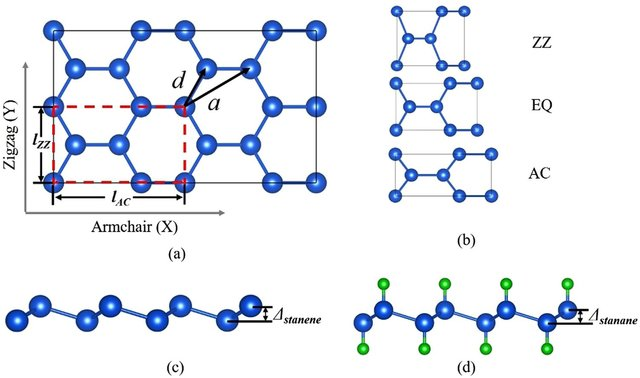
\includegraphics[width=17cm]{./gambar/struktur stanene.jpg}
    \caption{struktur dari material 2D stanene \citep{lu2017}}
    \label{struktur stanene}
\end{figure}
Stanene, bahan yang berasal dari timah (Sn) dalam bentuk lapisan dua dimensi dengan struktur yang mirip dengan graphene, telah menarik perhatian yang signifikan dalam beberapa tahun terakhir karena potensi aplikasinya dalam teknologi elektronik masa depan. Stanene pertama kali diusulkan oleh \citep{He2019} sebagai material topologis yang memiliki sifat konduktivitas elektronik yang luar biasa pada suhu kamar . Sifat ini berasal dari topologi elektroniknya yang memungkinkan pergerakan elektron tanpa hambatan di sepanjang tepinya, yang membuatnya sangat menarik untuk aplikasi dalam elektronik berenergi rendah .

Pada dasarnya, stanene adalah salah satu dari material topological insulator, di mana interior material berfungsi sebagai insulator sementara permukaannya mendukung arus listrik tanpa disipasi energi yang signifikan. Karakteristik unik ini disebabkan oleh adanya interaksi spin-orbit yang kuat pada atom timah, yang menyebabkan pembalikan pita energi dan pembentukan edge states yang terproteksi topologis . Penelitian eksperimental oleh \citep{zhu2015} menunjukkan bahwa stanene juga memiliki potensi sebagai bahan untuk transistor yang dapat beroperasi pada suhu kamar dengan efisiensi energi yang lebih tinggi dibandingkan dengan bahan konvensional seperti silikon.

Sifat-sifat unik stanene, seperti efek Hall kuantum spin (Quantum Spin Hall Effect), dihasilkan dari interaksi spin-orbit yang kuat pada atom timah. Ini menghasilkan pembalikan pita energi yang penting dalam pembentukan state topologi yang terlokalisasi di tepi material . Penelitian oleh \citep{PhysRevLett.111.136804} menunjukkan bahwa stanene, dengan struktur bandnya yang khas, dapat menghasilkan edge states yang dilindungi oleh simetri topologi, memungkinkan transportasi elektronik tanpa disipasi energi yang signifikan.

\citep{niuniu2022} melanjutkan dengan menggunakan DFT untuk mengeksplorasi bagaimana doping dengan elemen-elemen seperti bismut atau antimon dapat memodifikasi sifat elektronik stanene. Mereka menemukan bahwa doping dapat membuka celah pita energi yang lebih besar dan meningkatkan stabilitas struktural material, yang penting untuk aplikasi dalam perangkat elektronik canggih. Penelitian lebih lanjut oleh \citep{wu2020} menggunakan DFT untuk mengkaji dampak tegangan mekanik pada stanene. Hasilnya menunjukkan bahwa penerapan tegangan tertentu dapat memperluas atau mempersempit celah pita energi stanene, memungkinkan penyesuaian sifat elektronik material untuk berbagai aplikasi.

Penelitian eksperimental yang dilakukan oleh \citep{zhu2015} menunjukkan bahwa lapisan stanene dapat diproduksi secara epitaksial pada berbagai substrat, membuka jalan untuk integrasi dalam teknologi sirkuit terpadu dan perangkat spintronik . Pengembangan lebih lanjut dalam metode sintesis dan manipulasi stanene diharapkan akan membuka peluang baru untuk aplikasi dalam perangkat elektronik dengan efisiensi energi yang lebih tinggi dan kinerja yang lebih baik dibandingkan dengan material konvensional seperti silikon.

\begin{figure}
    \centering
    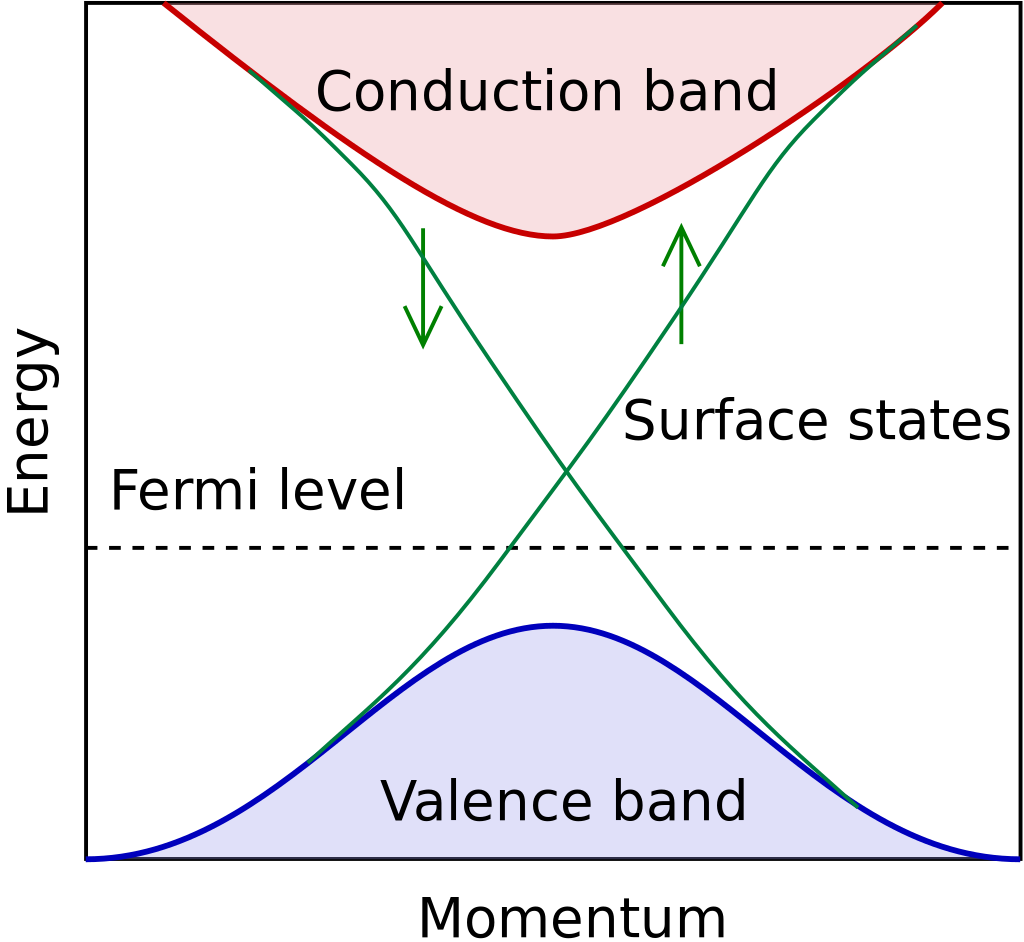
\includegraphics[width=10cm]{gambar/Topological_insulator_band_structure.png}
    \caption{Stuktur pita yang ideal untuk isolator topologi simetris pembalikan waktu 3D. Tingkat Fermi berada dalam celah pita bulk yang dilalui oleh kondisi permukaan Dirac bertekstur spin yang terlindungi secara topologis.}
    \label{band gap isolator topologis}
\end{figure}



%=====================================================================
\section{Teori Fungsional Densitas (\textit{Density Functional Theory})}
%=====================================================================
Salah satu kunci perkembangan sains dan teknologi adalah bagaimana kita bisa memahami dan mengatur sifat dari material dalam skala atom dan molekul secara individual. \textit{Density Functional Theory} (DFT) menjadi pendekatan yang sukses dalam penentuan solusi persamaan fundamental dalam fisika kuantum, yaitu persamaan \schro. DFT berkembang sangat pesat, dari sebuah teori yang digunakan sebagaian kecil oleh fisikawan menjadi dasar praktis bagi penelitian berbasis ilmu material, kimia, geologi, dll. Secara garis besar DFT merupakan teori tentang energi total, densitas elektron, dan relasinya dengan keadaan dasar (\textit{ground state}).

\subsection{Persamaan \schro}
Persamaan Schrödinger dikembangkan oleh fisikawan Austria bernama Erwin Schrödinger pada tahun 1925. Persamaan ini menyajikan fondasi teoretis yang kuat untuk memahami struktur elektron di atom dan memprediksi spektrum energi mereka. Persamaan ini berdasarkan pada konsep bahwa partikel subatom memiliki sifat gelombang dan partikel secara bersamaan. Dengan kata lain, persamaan Schrödinger menggambarkan partikel sebagai fungsi gelombang yang berubah seiring waktu. 
\begin{equation}
i\hbar \frac{\partial \Psi(\mathbf{r}, t)}{\partial t} = -\frac{\hbar^2}{2m} \nabla^2 \Psi(\mathbf{r}, t) + V(\mathbf{r})\Psi(\mathbf{r}, t)
\end{equation}

Namun, ketika kita mencoba mengaplikasikan persamaan Schrödinger pada sistem ril yang melibatkan banyak inti dan elektron, tantangan yang kompleks muncul. Salah satu masalah utamanya adalah ketidakmampuan untuk menyelesaikan persamaan tersebut secara analitik. Pada tahun 1929 \citeauthor{dirac1929quantum} mengatakan bahwa teori umum kuantum sudah hampir lengkap, namun kendalanya ialah mengaplikasikan teori-teori tersebut ke dalam sistem sebenarnya. Dalam kasus atom hidrogen sederhana, kita dapat menemukan solusi analitik untuk persamaan Schrödinger, tetapi ketika kita melibatkan lebih dari satu inti dan lebih dari satu elektron, solusi analitiknya menjadi tidak layak atau bahkan tidak ada.

Untuk kasus \textit{many-body \schro} \textit{equation}, Sistem atom yang kita miliki menyumbangkan potensial yang banyak serta fungsi gelombang yang rumit, karena dalam persamaan Schrödinger, fungsi eigen gelombang yang diperoleh haruslah unik dan simultan untuk semua koordinat inti maupun elektron. Kenyataannya kita perlu mendefinisikan potensial akibat interaksi elektron-elektron, inti-inti, dan elektron-inti. Sehingga Hamiltonian sistem memiliki bentuk
\begin{equation}
\hat{H} = -\sum_{i=1}^N \dfrac{\hbar^2}{2m_e}\nabla_i-\sum_{i=1}^M \dfrac{\hbar^2}{2M_I}\nabla_I^2+\dfrac{1}{2}\sum_{i\neq j}\dfrac{e^2}{4\pi \varepsilon_0}\dfrac{1}{|\mathbf{r_i}-\mathbf{r_j}|}+\dfrac{1}{2}\sum_{I\neq J}\dfrac{e^2}{4\pi \varepsilon_0}\dfrac{Z_IZ_J}{|\mathbf{R_I}-\mathbf{R_J}|}+\dfrac{1}{2}\sum_{i,I}\dfrac{e^2}{4\pi \varepsilon_0}\dfrac{Z_I}{|\mathbf{r_I}-\mathbf{R_I}|}.
\end{equation}
Kendala lainnya adalah interaksi kuantum antara partikel-partikel dalam sistem ril. Karena sifat kuantumnya, partikel-partikel ini saling terkait secara tidak terpisahkan dan mempengaruhi satu sama lain melalui potensial elektromagnetik. Interaksi semacam ini sulit diuraikan dengan tepat dalam bentuk matematika yang dapat dipecahkan. Sebagai hasil dari kompleksitas ini, para ilmuwan sering harus menggunakan metode pendekatan numerik dan komputasi yang canggih untuk memecahkan persamaan Schrödinger pada sistem ril.

Salah satu upaya yang dilakukan agar hamiltonian pada persamaan 2.2 terlihat lebih ramping adalah dengan mengaplikasikan sistem satuan Hartree \citep{hartree1928wave}. Teknik ini dikenal dengan istilah nondimensionalisasi. Dalam satuan Hartree, besaran seperti $m_e$, $\hbar$, $e$, dan $4\pi\varepsilon_0$ disubstitusikan dengan nilai 1. Nondimensioanlisasi dalam fisika matematika adalah proses mengubah persamaan diferensial atau perhitungan fisika menjadi bentuk yang tidak mengandung satuan pengukuran. Dalam konteks persamaan Schrödinger dan satuan Hartree, nondimensioanlisasi dilakukan dengan tujuan untuk menghilangkan faktor skala dari persamaan, sehingga memudahkan analisis dan perhitungan numerik, serta mengungkapkan hubungan yang lebih mendasar antara variabel yang terlibat.
\begin{equation}
\left[-\sum_{i=1}^N \nabla_i^2-\sum_{I=1}^M \frac{1}{2M_I}\nabla_I^2+\frac{1}{2}\sum_{i\neq j}\frac{1}{|\mathbf{r_i}-\mathbf{r_j}|}+\frac{1}{2}\sum_{I\neq J}\frac{Z_I Z_J}{|\mathbf{R_I}-\mathbf{R_J}|}-\sum_{i,I}\frac{Z_I}{|\mathbf{r_i}-\mathbf{R_I}|} \right]\Psi=E\Psi
\end{equation}
Ini adalah bentuk persamaan \textit{many-body \schro} yang paling umum digunakan untuk
pemodelan \textit{first-principles} material \citep{Guistino}. Persamaan ini menunjukkan dengan sangat jelas bahwa satu-satunya
parameter eksternal yang diperlukan dalam pendekatan ini adalah nomor atom, $Z_I$, dan
massa atom, $M_I$.

\subsection{Aproksimasi Born-Oppenheimer}
Teori Born-Oppenheimer \citep{oppenheimer1927zur} adalah suatu pendekatan fundamental dalam fisika molekul yang memungkinkan kita untuk memahami interaksi antara inti atom dan elektron secara terpisah. Pendekatan ini mendasarkan pada asumsi bahwa inti inti atom jauh lebih berat dan bergerak lebih lambat dibandingkan elektron, sehingga inti-inti atom dianggap sebagai partikel yang diam atau praktis tidak bergerak selama proses perubahan konfigurasi elektron.
Dasar teori Born-Oppenheimer mengacu pada fakta bahwa massa inti atom jauh lebih besar daripada massa elektron. Oleh karena itu, gerakan inti atom dalam molekul berlangsung secara lambat dan dalam skala waktu yang jauh lebih besar dibandingkan gerakan elektron. Dalam konteks ini, inti atom dianggap sebagai "titik" yang diam pada posisi tertentu sementara perubahan konfigurasi elektron terjadi. Selain itu jarak antar inti sangatlah besar sehingga Persamaan \schro dengan aproksimasi Born-Oppenheimer berubah menjadi.
\begin{equation}
\left[-\sum_{i=1}^N \nabla_i^2+\frac{1}{2}\sum_{i\neq j}\frac{1}{|\mathbf{r_i}-\mathbf{r_j}|}-\sum_{i,I}\frac{Z_I}{|\mathbf{r_i}-\mathbf{R_I}|} \right]\Psi=E\Psi
\end{equation}
Terlihat bahwa kita mencoret bentuk energi kinetik inti dan interaksi antar inti-inti. Persamaan ini adalah persamaan fundamental dalam sifat elektronik material.

Dengan menggunakan teori Born-Oppenheimer, kita dapat memisahkan persamaan Schrödinger keseluruhan untuk sistem molekul menjadi dua bagian terpisah. Pertama, kita menyelesaikan persamaan Schrödinger untuk elektron dengan mengabaikan perubahan posisi inti, menganggap inti-inti atom sebagai tetap pada posisi mereka. Hasil dari solusi ini memberikan distribusi elektron yang menggambarkan bentuk dan sifat orbital elektron di sekitar inti-inti atom. Selanjutnya, setelah mendapatkan distribusi elektron, kita dapat menyelesaikan persamaan Schrödinger kedua untuk gerakan inti atom dengan mengabaikan perubahan distribusi elektron saat inti bergerak. Solusi dari persamaan ini memberikan informasi tentang perubahan energi potensial yang dialami oleh inti atom ketika berada pada posisi tertentu. Kaitannya dengan perkembangan DFT, teori Born-Oppenheimer memainkan peran yang sangat penting. DFT adalah pendekatan teoretis dalam fisika kuantum yang digunakan untuk menghitung distribusi elektron dan sifat-sifat sistem many-elektron. Pendekatan ini berfokus pada densitas elektron sebagai variabel sentral.

\subsection{Teorema Hohenberg-Kohn}
Teorema Hohenberg-Kohn \citep{hohenberg1964inhomogeneous} adalah salah satu pilar fundamental dalam Teori Fungsional Densitas (DFT) dalam kimia kuantum dan fisika zat padat. Teorema ini pertama kali dirumuskan oleh Pierre Hohenberg dan Walter Kohn pada tahun 1964. Teorema ini menyediakan dasar konseptual yang mendasari pendekatan DFT dalam memahami dan menghitung sifat-sifat sistem banyak elektron.

Teorema Hohenberg-Kohn dibentuk dari 3 premis dasar \citep{Kurth_2005}, yaitu
\begin{enumerate}
    \item Densitas elektron pada keadaan dasar dari sistem dengan elektron yang salinng berinteraksi menentukan secara unik potensial eksternal $V_n(r)$.
    \item Energi keadaan dasar $E_0$ dan densitas keadaan dasar $n_0(r)$ dari sistem dibentuk dari potensial $v_0(r)$ yang dapat diperoleh dari prinsip variasi yang hanya melibatkan densitas elektron. Dalam kata lain kita dapat membentuk energi keadaan dasar sebagai fungsional dari densitas elektron $E_{vo}[n]$.
    \item Ada fungsional $F[n]$ sedemikian sehingga fungsional energi dapat ditulis sebagai
    \begin{equation}
        E_{v_0}[n]=F[n]+\int d^3rv_0(\mathbf{r})n(\mathbf{r})
    \end{equation}
\end{enumerate}
Teorema Hohenberg-Kohn memberikan dasar bagi pendekatan praktis dalam perhitungan DFT. Sebagai konsekuensinya, perhitungan DFT dapat difokuskan pada pencarian densitas elektron yang memberikan energi total minimum, daripada mencoba menemukan dan menyelesaikan fungsi gelombang banyak elektron yang rumit. Dengan kata lain, permasalahan minimisasi densitas dalam DFT dapat dianggap setara dengan menemukan densitas yang memenuhi teorema Hohenberg-Kohn dan memberikan energi total yang paling rendah.

%=====================================================================
\subsection{Persamaan Kohn-Sham}
%=====================================================================
Tahap terakhir dari aproksimasi-aproksimasi yang telah dipertimbangkan dalam upaya penyederahaan persamaan \schro adalah dengan membentuk persamaan kohn-sham yang dikenalkan oleh \citeauthor{kohnsham} dalam artikelnya yang berjudul "\textit{Self-Consistent Equations Including Exchange and Correlation Effects}". Dalam aproksimasi sebelumnya, kita telah mempertimbangkan tolakan Coulomb antar elektron dengan elektrodinamika klasik, dan menambahkan interaksi \textit{exchange} antar elektron untuk memenuhi sifat kuantum elektron. Namun kita perlu menambah dua bentuk potensial lagi yaitu potensial korelasi antar elektron dan potensial pertukaran elektron, Sehingga bentuk hamiltonian akan berubah menjadi:
\begin{equation}
\left [\dfrac{\nabla^2_i}{2}-V_n(\mathbf{r})+V_H(\mathbf{r})+V_{XC}(\mathbf{r})  \right]\phi_i=\varepsilon_i\phi_i(\mathbf{r})
\end{equation}

namun dalam persamaan di atas kita belum tau secara pasti potensial korelasi dan pertukaran, oleh karena itu dikembangkan pula aproksimasi untuk mendekati nilai potensial korelasi dan pertukaran yang sebenarnya. persamaan kohm-sham ini dapat diselesaikan dengan siklus perhitungan \textit{self-consistent field} (SCF). 

\subsection{Fungsional \textit{Exchange-Correlation}}
Untuk menyelesaiakan persamaan Kohn-Sham, kita perlu mendefinisikan fungsional Pertukaran-Korelasi (\textit{Exchange-Correlation}) $E_{XC}[\Psi_i]$. Fungsional \textit{Exchange-Correlation} adalah salah satu komponen kunci dalam DFT. Fungsional ini mencerminkan kompleksitas interaksi elektron-elektron dalam sistem \textit{many-body}, di mana pertukaran menggambarkan efek statistik partikel dan korelasi menggambarkan efek kuantum pada distribusi spasial elektron. Pada persamaan 2.6, dengan mendefinisikan $E_{XC}$ yang sesuai, kita dapat memperoleh $V_{XC}$ melalui hubungan berikut
\begin{equation}
V_{XC}=\frac{\delta E_{XC}}{\delta n(\mathbf{r})}
\end{equation}
Fungsional Pertukaran-Korelasi merujuk pada pendekatan untuk menghitung energi total sistem berdasarkan distribusi kepadatan elektronnya. Energi total ini terdiri dari beberapa kontribusi, salah satunya adalah energi pertukaran-korelasi, yang umumnya dipecah menjadi dua bagian yaitu energi pertukaran dan energi korelasi. Energi pertukaran muncul karena prinsip eksklusi Pauli, di mana elektron-elektron dengan spin yang sama tidak dapat memiliki keadaan kuantum yang sama. Oleh karena itu, elektron-elektron dalam sistem "menukar tempat" secara statistik untuk menghindari keadaan energi yang lebih tinggi. Energi pertukaran ini dapat diperkirakan dengan menggunakan berbagai pendekatan.
Dalam upaya untuk mengatasi keterbatasan aproksimasi pada fungsional pertukaran-korelasi, sudah banyak jenis pendekatan umum telah dikembangkan oleh ilmuwan, salah satunya adalah Pendekatan \textit{local density approximation} (LDA) dan \textit{generelized gradient approximation} (GGA).

\begin{figure}
    \centering
    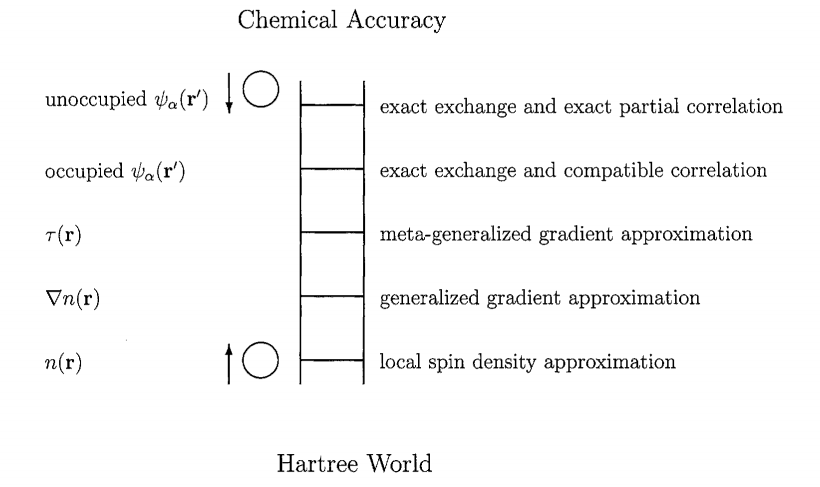
\includegraphics[width=12cm]{./gambar/tangga yakub.png}
    \caption{Skema \textit{Jacob's Ladders} yang dipopulerkan oleh \citeauthor{Perdew} yang menggambarkan tingkat akurasi fungsional dari terendah hingga tertinggi.}
    \label{fig:kpoints}
\end{figure}

Pendekatan LDA merupakan salah satu pendekatan awal dalam teori DFT, yang mempertimbangkan energi pertukaran-korelasi sebagai fungsi dari kepadatan elektron lokal pada setiap titik dalam ruang. LDA sederhana dan efisien dalam banyak kasus, tetapi sering kali tidak mampu menangkap efek kuantum yang lebih kompleks, seperti interaksi antara elektron yang lebih jauh. Sementara itu GGA merupakan perkembangan lebih lanjut dari LDA, di mana energi pertukaran-korelasi dinyatakan sebagai fungsi dari gradien kepadatan elektron. Pendekatan ini mempertimbangkan perubahan kepadatan elektron di seluruh sistem, memungkinkan pengambilan data spasial yang lebih baik dan hasil yang lebih akurat, terutama dalam kasus di mana interaksi antara elektron jarak jauh berperan signifikan.

Kedua kelas pendekatan ini, LDA dan GGA, memiliki kelebihan dan keterbatasan masing-masing dalam mengestimasi energi pertukaran-korelasi. Pemilihan pendekatan yang tepat tergantung pada sistem yang sedang diinvestigasi dan tingkat akurasi yang diinginkan dalam perhitungan kimia kuantum. Pada dasarnya, fungsional pertukaran-korelasi membantu mengkonversi distribusi kepadatan elektron ke dalam energi total sistem, memungkinkan simulasi komputasi yang akurat tentang sifat kimia, fisika, dan sifat material. Pengembangan fungsional pertukaran-korelasi yang lebih baik menjadi fokus dalam penelitian kimia kuantum, karena pengaruhnya terhadap keakuratan hasil perhitungan dalam berbagai konteks, mulai dari struktur molekul hingga reaksi kimia kompleks.
Dalam praktiknya, para ilmuwan sering menggunakan pendekatan dan aproksimasi yang berbeda dalam mengembangkan fungsional pertukaran-korelasi baru, karena tidak ada pendekatan yang sempurna untuk mengatasi kompleksitas interaksi elektron dalam sistem \textit{many-body}. Oleh karena itu, pemahaman tentang fungsional pertukaran-korelasi memiliki dampak signifikan dalam interpretasi hasil perhitungan teori densitas dan dalam pengembangan material dan senyawa baru dengan sifat-sifat unik.

%=====================================================================
\section{Quantum ESPRESSO}
%=====================================================================
\begin{figure}
    \centering
    
\includegraphics[width=10cm]{./gambar/qelogo.png}
    \caption{Logo Quantum ESPRESSO}
    \label{fig:kpoints}
\end{figure}
Quantum ESPRESSO adalah perangkat lunak simulasi fisika yang memungkinkan pengguna untuk melakukan perhitungan teoritis tentang sifat elektronik dan atomik material menggunakan metode mekanika kuantum. Perangkat lunak ini dikembangkan oleh sebuah tim internasional ahli dalam bidang fisika teoritis dan komputasi, dan dirilis sebagai proyek \textit{open source} yang tersedia secara gratis untuk digunakan oleh siapa saja. Tujuan utama dari Quantum ESPRESSO adalah untuk menyediakan alat yang dapat digunakan untuk memahami dan meramalkan sifat bahan secara lebih akurat dan efisien daripada metode eksperimental yang mahal dan rumit. Dalam upaya untuk mencapai tujuan ini, Quantum ESPRESSO menggunakan berbagai teknik mekanika kuantum, termasuk teori fungsional densitas (DFT), yang memungkinkan pengguna untuk memodelkan dan memprediksi sifat material seperti struktur kristal, energi ikatan, dan spektrum elektronik.

Quantum ESPRESSO dirancang untuk digunakan oleh para ilmuwan dan peneliti di berbagai bidang, termasuk fisika, kimia, dan teknik material. Perangkat lunak ini dapat digunakan untuk mempelajari berbagai jenis material, seperti logam, senyawa, dan material organik. Dalam pengembangan dan penggunaan Quantum ESPRESSO, para peneliti dapat menghasilkan pemahaman yang lebih baik tentang sifat material yang kompleks, memprediksi sifat material baru, dan mempercepat pengembangan teknologi baru. Quantum ESPRESSO memiliki beberapa fitur dan komponen penting yang memungkinkan pengguna untuk melakukan simulasi fisika dan analisis material. Salah satu fitur utama dari Quantum ESPRESSO adalah Modul PWSCF (\textit{Plane-Wave Self-Consistent Field}), yang menyediakan algoritma yang efisien untuk memecahkan persamaan \schro yang rumit dan memprediksi sifat elektronik material. Selain itu, Quantum ESPRESSO juga memiliki modul untuk memprediksi sifat getaran kristal, dinamika molekuler, dan sifat termodinamika material.

Dengan Quantum ESPRESSO, para ilmuwan dapat menghasilkan hasil simulasi dan analisis yang sangat berguna dan dapat dimanfaatkan dalam berbagai aplikasi. Misalnya, Quantum ESPRESSO dapat digunakan untuk merancang bahan baru dengan sifat khusus, seperti kekuatan yang lebih tinggi atau kemampuan konduktivitas listrik yang lebih baik. Selain itu, Quantum ESPRESSO dapat digunakan untuk mempelajari sifat material dalam kondisi yang ekstrem, seperti suhu dan tekanan yang sangat tinggi atau rendah. Secara keseluruhan, Quantum ESPRESSO adalah alat yang sangat berguna bagi para ilmuwan dan peneliti yang tertarik dalam memahami sifat material secara lebih mendalam dan meramalkan sifat material baru yang belum terungkap. Dengan penggunaan Quantum ESPRESSO, para ilmuwan dapat mempercepat pengembangan teknologi baru dan memberikan kontribusi yang signifikan dalam pemahaman kita tentang dunia material. 




\newpage

    %%%%%%%%%%%%%%%%%%%%%%%%%%%%%%%%%%%%%%%%%%%%%%%%%%%%%%%%%%%%%%%%%%%%%%
% BAB METODOLOGI
%=====================================================================
\renewcommand{\thechapter}{\Roman{chapter}}
\addtocontents{toc}{\vskip10pt}
\chapter{METODOLOGI}
\renewcommand{\thechapter}{\arabic{chapter}}
%---------------------------------------------------------------------

%=====================================================================
\section{Diagram Alir Penelitian}
%=====================================================================

Dalam konteks penelitian ini, penting untuk menyadari bahwa pencapaian hasil yang berkualitas dan signifikan melibatkan proses yang terstruktur dan sistematis. Progres yang efektif dalam eksplorasi masalah penelitian didasarkan pada langkah-langkah yang diatur secara terencana dan berkesinambungan. Oleh karena itu, penelitian ini menjelaskan dan mengikuti serangkaian tahapan yang saling terkait, yang dirinci secara kronologis dan terurai dalam diagram alir yang dapat dilihat pada Gambar 3.1.

\begin{figure}
    \centering
    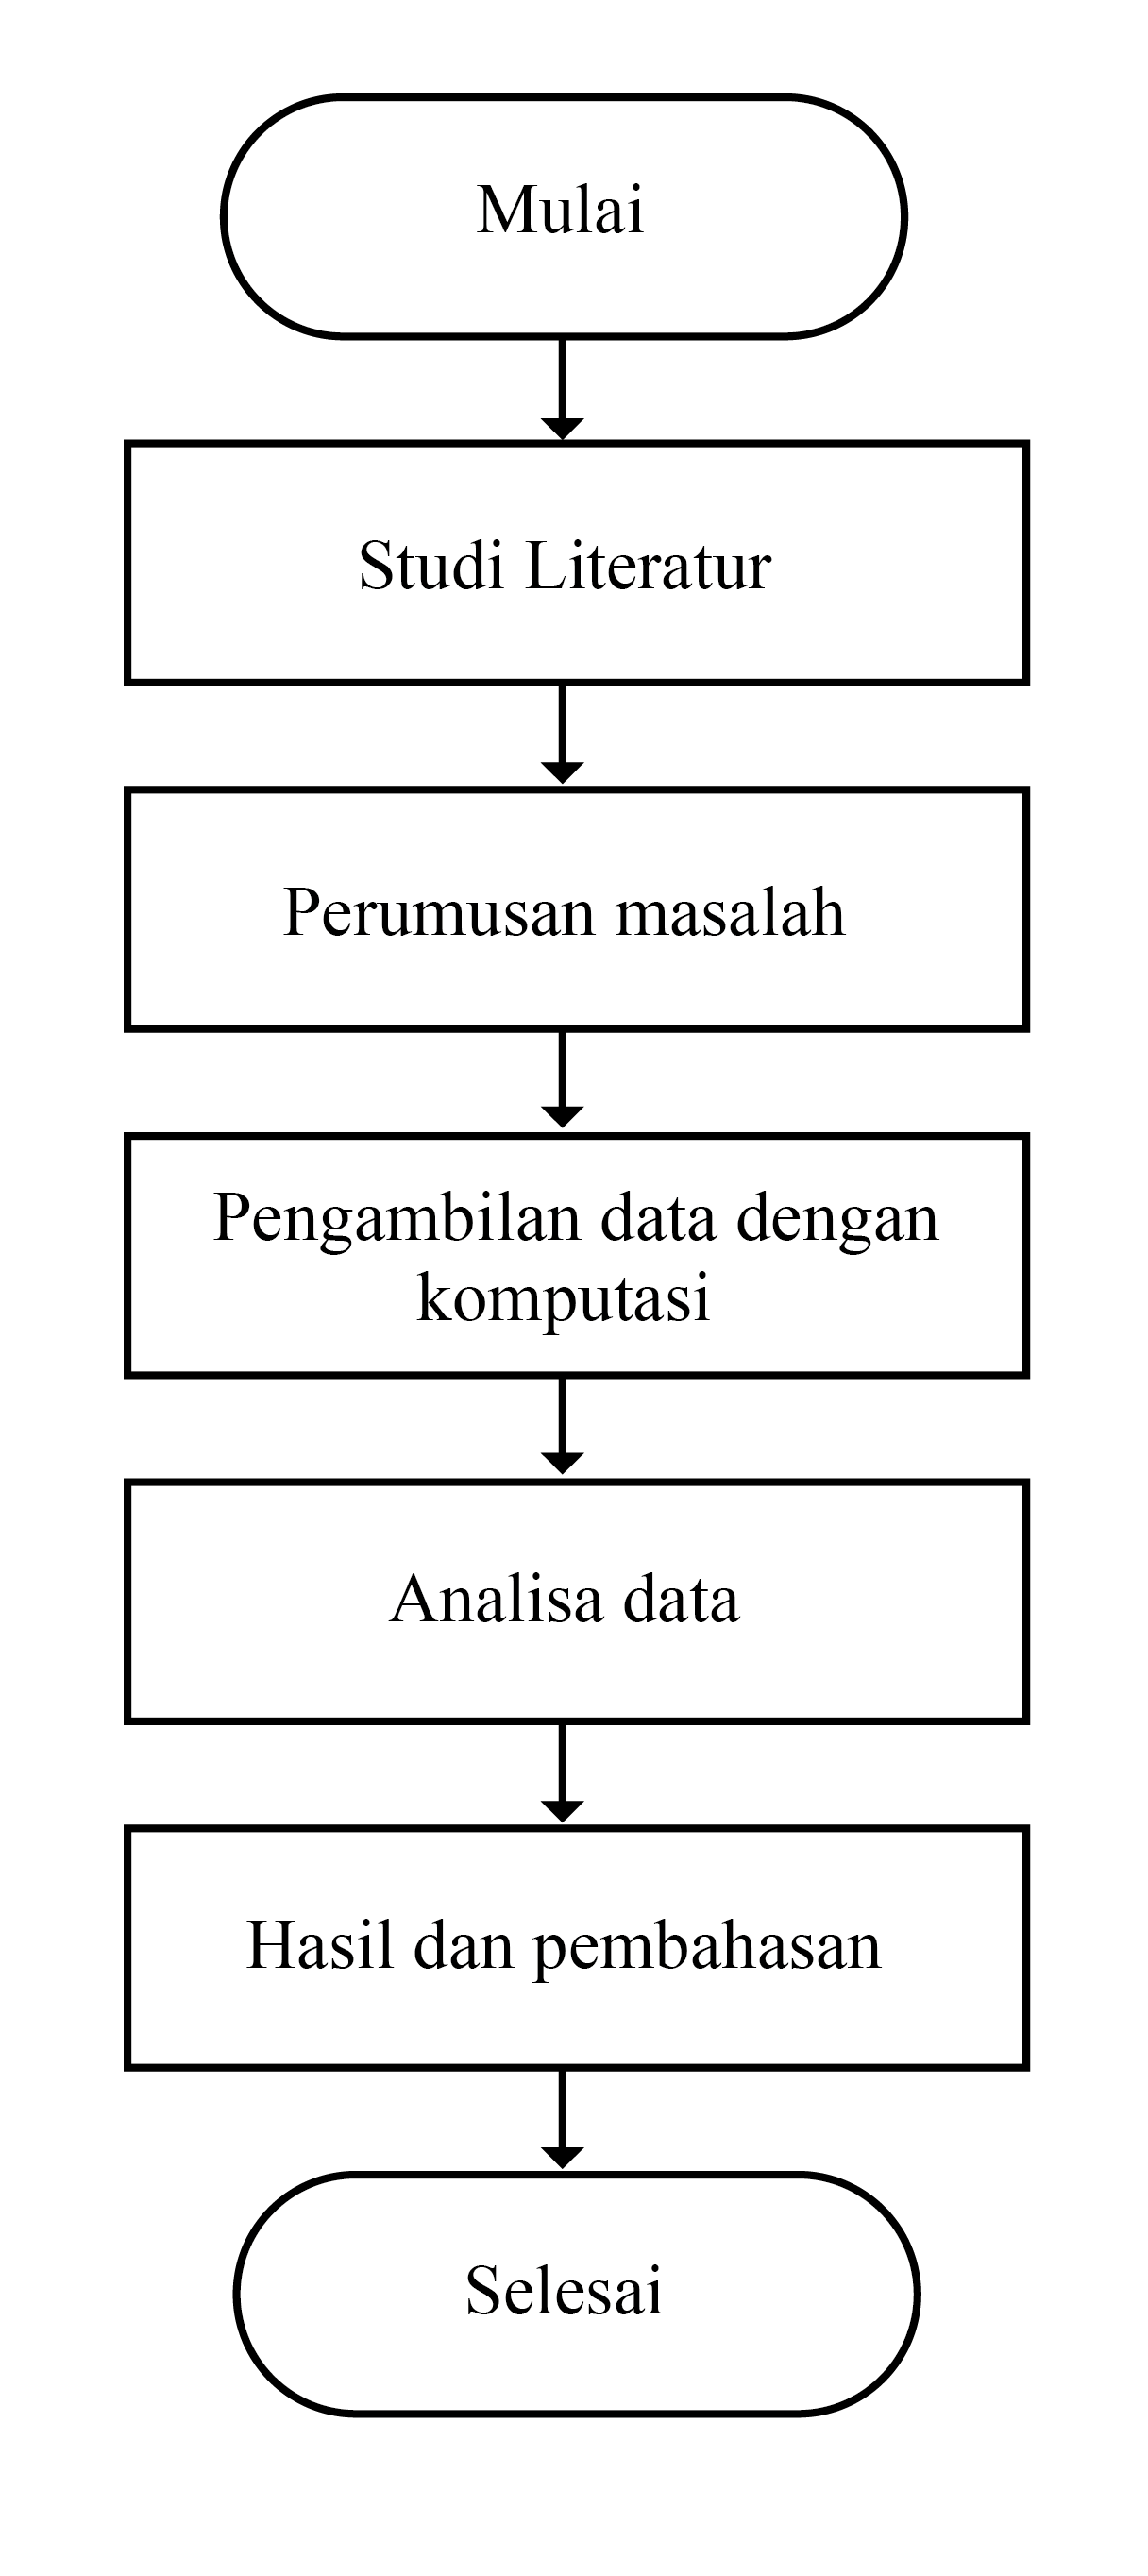
\includegraphics[width=5cm]{gambar/Flowchart Kegiatan.png}
    \caption{Diagram Alir Penelitian}
\end{figure}

%=====================================================================
\section{Jenis dan Desain Penelitian}
%=====================================================================
Pada penelitian ini jenis penelitian yang digunakan adalah penelitian komputasi, yaitu penelitian yang dilakukan di dalam komputer dengan metode pemodelan mekanika kuantum komputasi untuk menyelidiki sifat elektronik pada Stanene 2-dimensi menggunakan perangkat lunak Quantum ESPRESSO.


%=====================================================================
\section{Lokasi dan Waktu Penelitian}
%=====================================================================
Penelitian ini dilakukan pada saat melakukan kerja praktik
dan bimbingan di Pusat Riset Fisika Kuantum, Badan Riset dan
Inovasi Nasional (BRIN) yang berlokasi di Kawasan Sains dan Teknologi (KST) B. J. Habibie, Serpong, Tangerang Selatan. Waktu pelaksanaan tugas akhir selama 1 bulan (7 januari 2023 - 31 Januari 2023). 

%=====================================================================

%---------------------------------------------------------------------

\subsection{Perangkat Penelitian}
%---------------------------------------------------------------------
Pada penelitian ini menggunakan perangkat komputer berupa laptop yang dimiliki oleh peneliti

%---------------------------------------------------------------------
\subsection{Prosedur Penelitian}
Dalam prosedur penelitian ini, kami secara komprehensif membahas perangkat yang telah digunakan untuk mendukung jalannya penelitian ini, serta merincikan langkah-langkah kerja yang kami lakukan dalam rangka mencapai tujuan yang telah ditetapkan. Pada tahap awal, kami akan memberikan gambaran mendalam tentang perangkat keras dan perangkat lunak yang menjadi tulang punggung eksperimen ini. Ini mencakup spesifikasi teknis dari komputer yang digunakan untuk menjalankan perhitungan, perangkat pendukung seperti ketersediaan sumber daya komputasi berkecepatan tinggi, dan perangkat lunak yang mendukung analisis dan pengolahan data.

Selanjutnya, dalam upaya kami untuk mewujudkan simulasi yang akurat dan konsisten, kami akan memaparkan detail komputasi yang digunakan sebagai dasar input untuk program Quantum ESPRESSO. Ini melibatkan parameter-parameter yang terlibat dalam setiap perhitungan, termasuk energi kinetik \textit{cut-off}, ukuran grid \texttt{K-POINTS}, dan jenis potensial yang digunakan. Penjelasan rinci ini akan memberikan pemahaman mendalam tentang pemilihan parameter dan konfigurasi tertentu yang kami terapkan dalam eksperimen ini.

Langkah demi langkah, kami akan menggambarkan proses komputasi yang diterapkan, dari persiapan input hingga eksekusi perhitungan, serta tahap analisis hasil yang dihasilkan. Dengan memberikan informasi yang lengkap dan rinci tentang seluruh prosedur komputasi, kami berharap bahwa penelitian ini akan lebih mudah diulang oleh pihak lain dan menghasilkan hasil yang konsisten serta dapat diverifikasi. Dengan demikian, bagian ini tidak hanya akan memberikan panduan praktis bagi pembaca yang ingin mengulangi eksperimen, tetapi juga menguraikan landasan kuat dari eksperimen kami yang memanfaatkan alat Quantum ESPRESSO untuk mendapatkan wawasan yang berharga dalam ranah penelitian ini. 
%---------------------------------------------------------------------

\vspace{3mm}

\subsubsection{Detail Komputasi}
Dalam penelitian ini digunakan \qe  sebagai perangkat lunak komputasi\citep{Giannozzi_2009}. Kami gunakan sel satuan untuk membentuk struktuk \textit{stanene}. Dengan variasi \texttt{ecutwfc} sebesar 60 Ry dan \texttt{K-POINTS} sebesar $24\times24\times1$ untuk membagi daerah Brillouin dengan kisi Monkhorst Pack (MP)\citep{MP}. Kedua nilai tersebut diperoleh dari uji konvergensi yang akan dijelaskan lebih lengkap pada BAB 4. Digunakan fungsional Perdew-Burke-Ernzerhof (PBE)\cite{PBE} sebagai \textit{generalized gradient approximation} (GGA) untuk melengkapi fungsi korelasi dan pertukaran. Potensial semu yang digunakan untuk menggambarkan elektron valensi dan elektron inti adalah\textit{projector augmented wave method} (PAW)\citep{PAW}. Selain itu, ruang vakum dibuat sebesar .

Diagram alir komputasi yang akan dilakukan dalam penelitian ini dapat dilihat pada Gambar \ref{FlowchartKomputasi}. Seluruh prosedur komputasi dalam Gambar \ref{FlowchartKomputasi} dilakukan dalam \qe. Sementara visualisasi data hasil komputasi dibuat dengan bantuan dari kode python menggunakan library matplotlib dan numpy yang dibuat di dalam VS code dengan jupyter notebook.
\begin{figure}
    \centering
    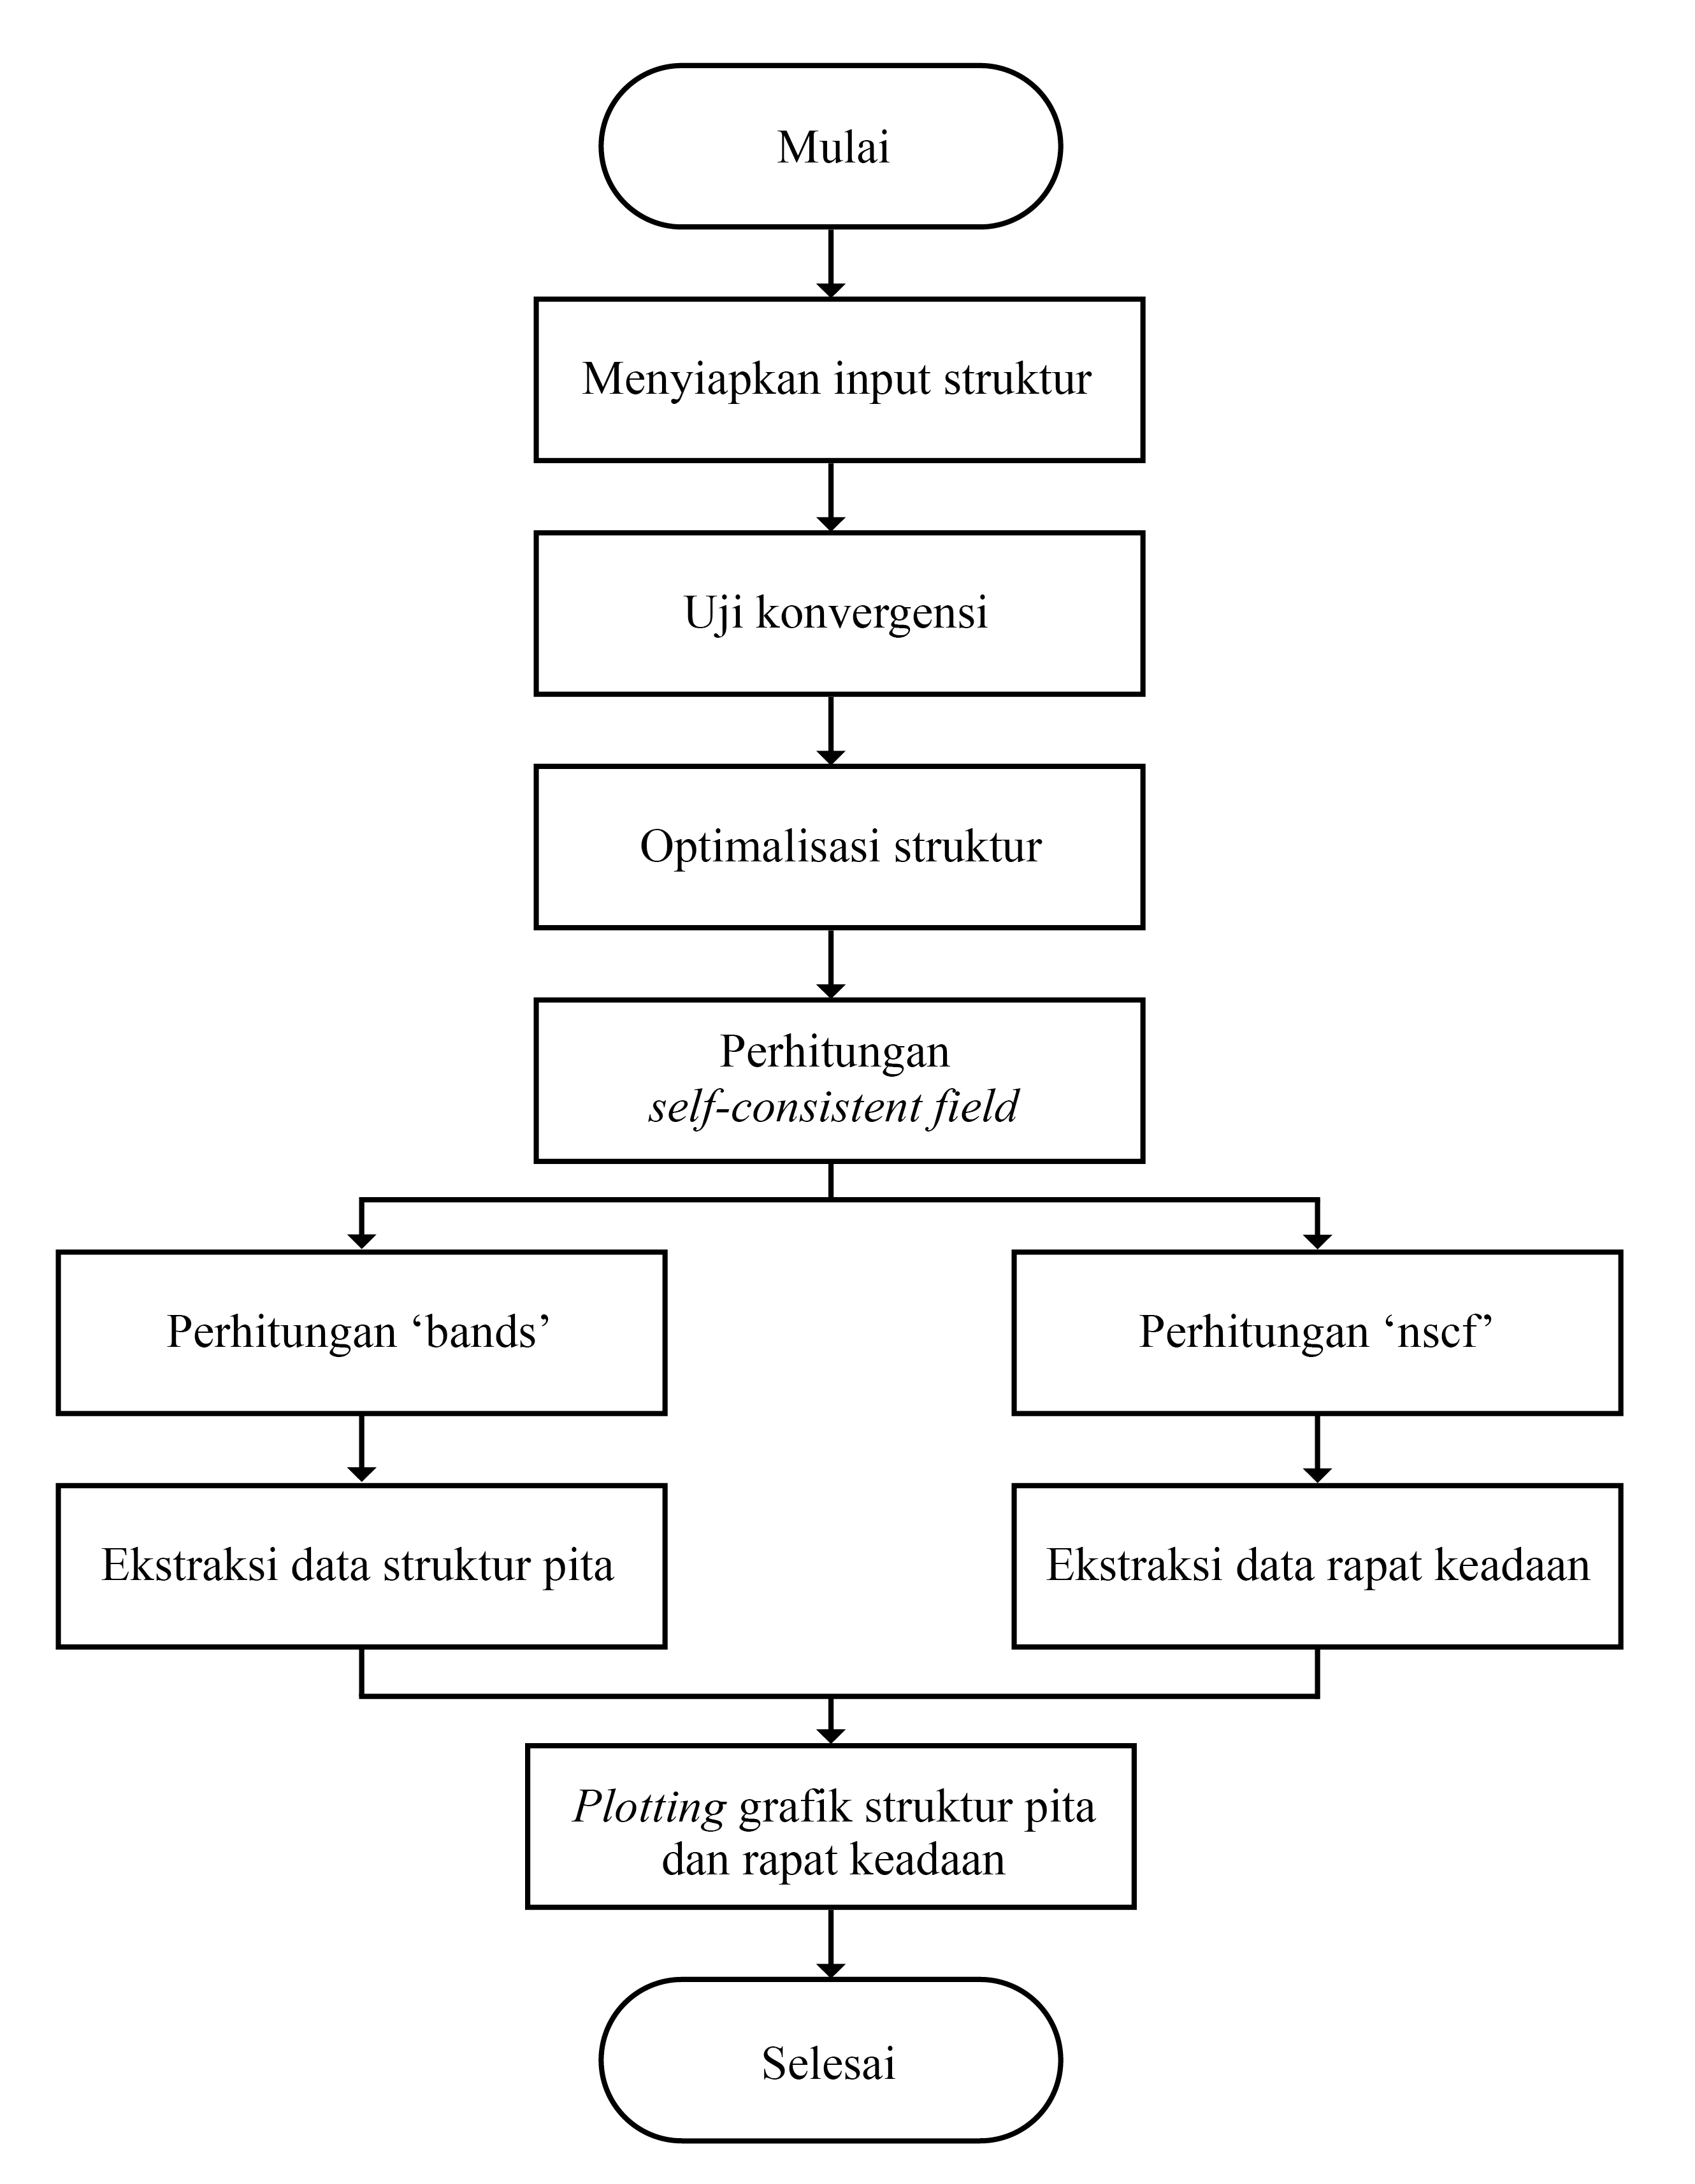
\includegraphics[width=12cm]{gambar/Flowchart Komputasi.png}
    \caption{Diagram alir komputasi}
    \label{FlowchartKomputasi}
\end{figure}

\subsubsection{Persiapan Struktur input}
Sebelum melakukan optimasi struktur, tentunya kita perlu membentuk material yang kita hendaki. Dalam penelitian ini terdapat 5 struktur yang akan dihitung sifat elektroniknya, dengan masing-masing struktur dijelaskan lebih lanjut di BAB 4. Untuk contoh kalkulasi dalam BAB ini, kami ambil struktur stanene. Secara garis besar ada 2 bagian penting dalam \textit{input} Quantum ESPRESSO yaitu \textit{Name Card}, dan \textit{Name List}. \textit{Name card} adalah file input utama dalam Quantum ESPRESSO yang mengandung semua informasi dasar tentang tugas perhitungan yang akan dilakukan. \textit{Name card} berisi informasi seperti tipe kisi, parameter elektronik, dan parameter lain yang spesifik untuk jenis perhitungan tertentu. Sedangkan \textit{Name list} adalah bagian dari \textit{name card} yang berisi kelompok parameter yang berhubungan dengan tugas perhitungan tertentu. \textit{Name list} dikelompokkan berdasarkan fungsinya dalam perhitungan. Misalnya, beberapa \textit{name list} yang umum dalam Quantum ESPRESSO adalah \texttt{CONTROL}, \texttt{SYSTEM}, \texttt{ELECTRONS}, \texttt{IONS}, dan sebagainya. Setiap namelist memiliki sejumlah parameter yang dapat disesuaikan untuk mengatur perilaku perhitungan.

File input stanene yang kami gunakan dapat dilihat sebagai berikut
\begin{lstlisting}
&control
calculation = 'scf'
prefix='stanene',
pseudo_dir = '../pseudo/',
outdir='../tmp/'
/
&system
ibrav = 4,
a=4.68
c=20,
nat = 2,
ntyp = 1,
ecutwfc = 60.0,
occupations = 'smearing'
smearing = 'm-p'
degauss = 0.02
/
&electrons
mixing_beta = 0.7
conv_thr = 1.0d-6
/
ATOMIC_SPECIES
Sn 118.710 Sn_pbe_v1.uspp.F.UPF
ATOMIC_POSITIONS (crystal)
Sn 0.333333333 0.666666666 0.500000000
Sn 0.666666666 0.333333333 0.500000000
K_POINTS {automatic}
24 24 1 0 0 0
\end{lstlisting}
input di atas merupakan input kalkulasi \texttt{scf}. Namelist \texttt{ibrav} berfungsi untuk mendefinisikan sistem kristal apa yang ingin kita gunakan. Dalam penelitian ini, kami menggunakan \texttt{ibrav}=4 yang mendefinisikan sistem kubik sebagai sel satuan. $a$, $b$, dan $c$ berturut-turut adalah besar vektor kisi pada arah sumbu $x$, $y$, dan $z$. Penentuan angka 4.68 dalam input diatas berdasarkan data parameter kisi stanene sebelumnya. Angka ini dipilih agar iterasi yang dilakukan tidak terlalu lama. Namelist \texttt{nat} mendefinisikan jumlah atom dalam sel yang kita bentuk sedangkan \texttt{ntyp} mendefinisikan berapa jenis atom dalam sel yang kita bentuk. namelist \texttt{ecutwfc} adalah energi kinetik \textit{cut-off} yang nilainya diperoleh melelaui uji konvergensi yang akan dijelaskan pada BAB selanjutnya.

\begin{table}[ht] % [h] menyatakan posisi. h: here, t: top, b: bottom
	\centering
	\caption{Kode-kode \texttt{ibrav} dalam Quantum ESPRESSO.}
	\label{tabel optimasi}
	\label{tab:ibrav}
\begin{tabular}{c c p{4cm} }
\hline
\textbf{Kode ibrav} & \textbf{Jenis Kisi} & \textbf{Sistem Kristal} \\
\hline
 1 & Kubik Primitif & $a=b=c$, $\alpha=\beta=\gamma=90^\circ$ \\
\hline
 2 & Kubik Berpusat pada Badan & $a=b=c$, $\alpha=\beta=\gamma=90^\circ$ \\
\hline
 3 & Kubik Berpusat pada Wajah & $a=b=c$, $\alpha=\beta=\gamma=90^\circ$ \\
\hline
 4 & Kubik Berpusat pada Ruang & $a=b=c$, $\alpha=\beta=\gamma=90^\circ$ \\
\hline
 5 & Tetragonal Primitif & $a=b\neq c$,  $\alpha=\beta=\gamma=90^\circ$ \\
\hline
 6 & Tetragonal Berpusat pada Badan & $a=b\neq c$,  $\alpha=\beta=\gamma=90^\circ$ \\
\hline
 7 & Ortorombik Primitif & $a\neq b\neq c$,  $\alpha=\beta=\gamma=90^\circ$ \\
\hline
 8 & Ortogonal Berpusat pada Badan & $a\neq b\neq c$,  $\alpha=\beta=\gamma=90^\circ$ \\
\hline
 9 & Ortogonal Berpusat pada Wajah & $a\neq b\neq c$, $\alpha=\beta=\gamma=90^\circ$ \\
\hline
 10 & Rhombohedral & $a=b=c$,  $\alpha=\beta=\gamma\neq90^\circ$ \\
\hline
 11 & Monoklinik Primitif & $a\neq b\neq c$,  $\alpha=\gamma=90^\circ, \beta\neq90^\circ$ \\
\hline
 12 & Monoklinik Berpusat pada Badan & $a\neq b\neq c$, $\alpha=\gamma=90^\circ, \beta\neq90^\circ$ \\
\hline
 13 & Trigonal Primitif & $a=b=c$, $\alpha=\beta=\gamma\neq90^\circ$ \\
\hline
 14 & Trigonal Berpusat pada Badan & $a=b=c$, $\alpha=\beta=\gamma\neq90^\circ$ \\
\hline
 15 & Trigonal Berpusat pada Wajah & $a=b=c$, $\alpha=\beta=\gamma\neq90^\circ$ \\
\hline
	\end{tabular}
\end{table}

Pada \texttt{ATOMIC\_SPECIES} terdapat jenis atom yang menyusun sel satuan yang kita bentuk, dalam hal ini untuk struktur stanene maka atom penyusun pad struktur hanyalah atom timah (Sn). Di samping lambang unsur, terdapat massa atom yang juga perlu didefinisikan serta \textit{pseduopotential} (potensial semu) yang akan digunakan. File \textit{pseudopotential} disimpan dalam direktori khusus agar mudah dipanggil dalam perhitungan untuk struktur lainnya.

\subsubsection{Uji Konvergensi}
Uji konvergensi adalah proses penting dalam perhitungan menggunakan paket perangkat lunak Quantum ESPRESSO untuk memastikan bahwa hasil perhitungan numerik sudah cukup akurat dan stabil. Ada dua parameter utama yang sering diuji untuk konvergensi \texttt{ecutwfc} dan \texttt{kpoints}. Parameter \texttt{ecutwfc} (\textit{energy cut-off for wave functions}) adalah nilai energi maksimum yang digunakan untuk memotong fungsi gelombang elektron. Nilai ini menentukan sejauh mana deret Fourier digunakan untuk merepresentasikan fungsi gelombang. Semakin tinggi nilai \texttt{ecutwfc}, semakin banyak komponen deret Fourier yang digunakan, yang pada gilirannya dapat meningkatkan akurasi hasil perhitungan. Sedangkan titik-titik k (\texttt{K-POINTS}) digunakan untuk menghitung integral di dalam ruang resiprok. Jumlah dan distribusi titik-titik k memiliki dampak pada akurasi hasil perhitungan, terutama untuk sifat-sifat terkait permukaan energi, densitas elektron, dan lainnya. Dalam penelitian ini, dilakukan siklus \texttt{scf} seperti yang ditampilkan dalam skema diagram alir 3.3, kami melakukan perhitungan dengan mencoba beberapa variasi \texttt{ecutwfc} dan melihat di nilai \texttt{ecutwfc} berapakah energi sistem mulai konvergen. Hal serupa dilakukan untuk menemukan konvergensi nilai \texttt{K-POINTS}.


\subsubsection{Optimasi Struktur}
Nilai konstanta kisi dan posisi atom dalam struktur input bukanlah posisi paling optimal. Oleh karena itu kita perlu melakukan relaksasi strukutur dengan menggunakan perintah kalkulasi \texttt{vc-relax}. \texttt{vc-relax} (\textit{Variable Cell Relaxation}) adalah kalkulasi untuk merelaksasi struktur kristal. Tujuan utamanya adalah untuk mencari konfigurasi struktur yang memiliki minimum energi total minimum, yang menggambarkan keadaan terstabilkan dari sistem kristal yang kita miliki.

Untuk melakukan kalkulasi \texttt{vc-relax}, input file Quantum ESPRESSO pada bagian \texttt{calculation} perlu didefinisikan sebagai
\begin{lstlisting}
calculation = 'vc-relax'
\end{lstlisting}

\begin{figure}
    \centering
    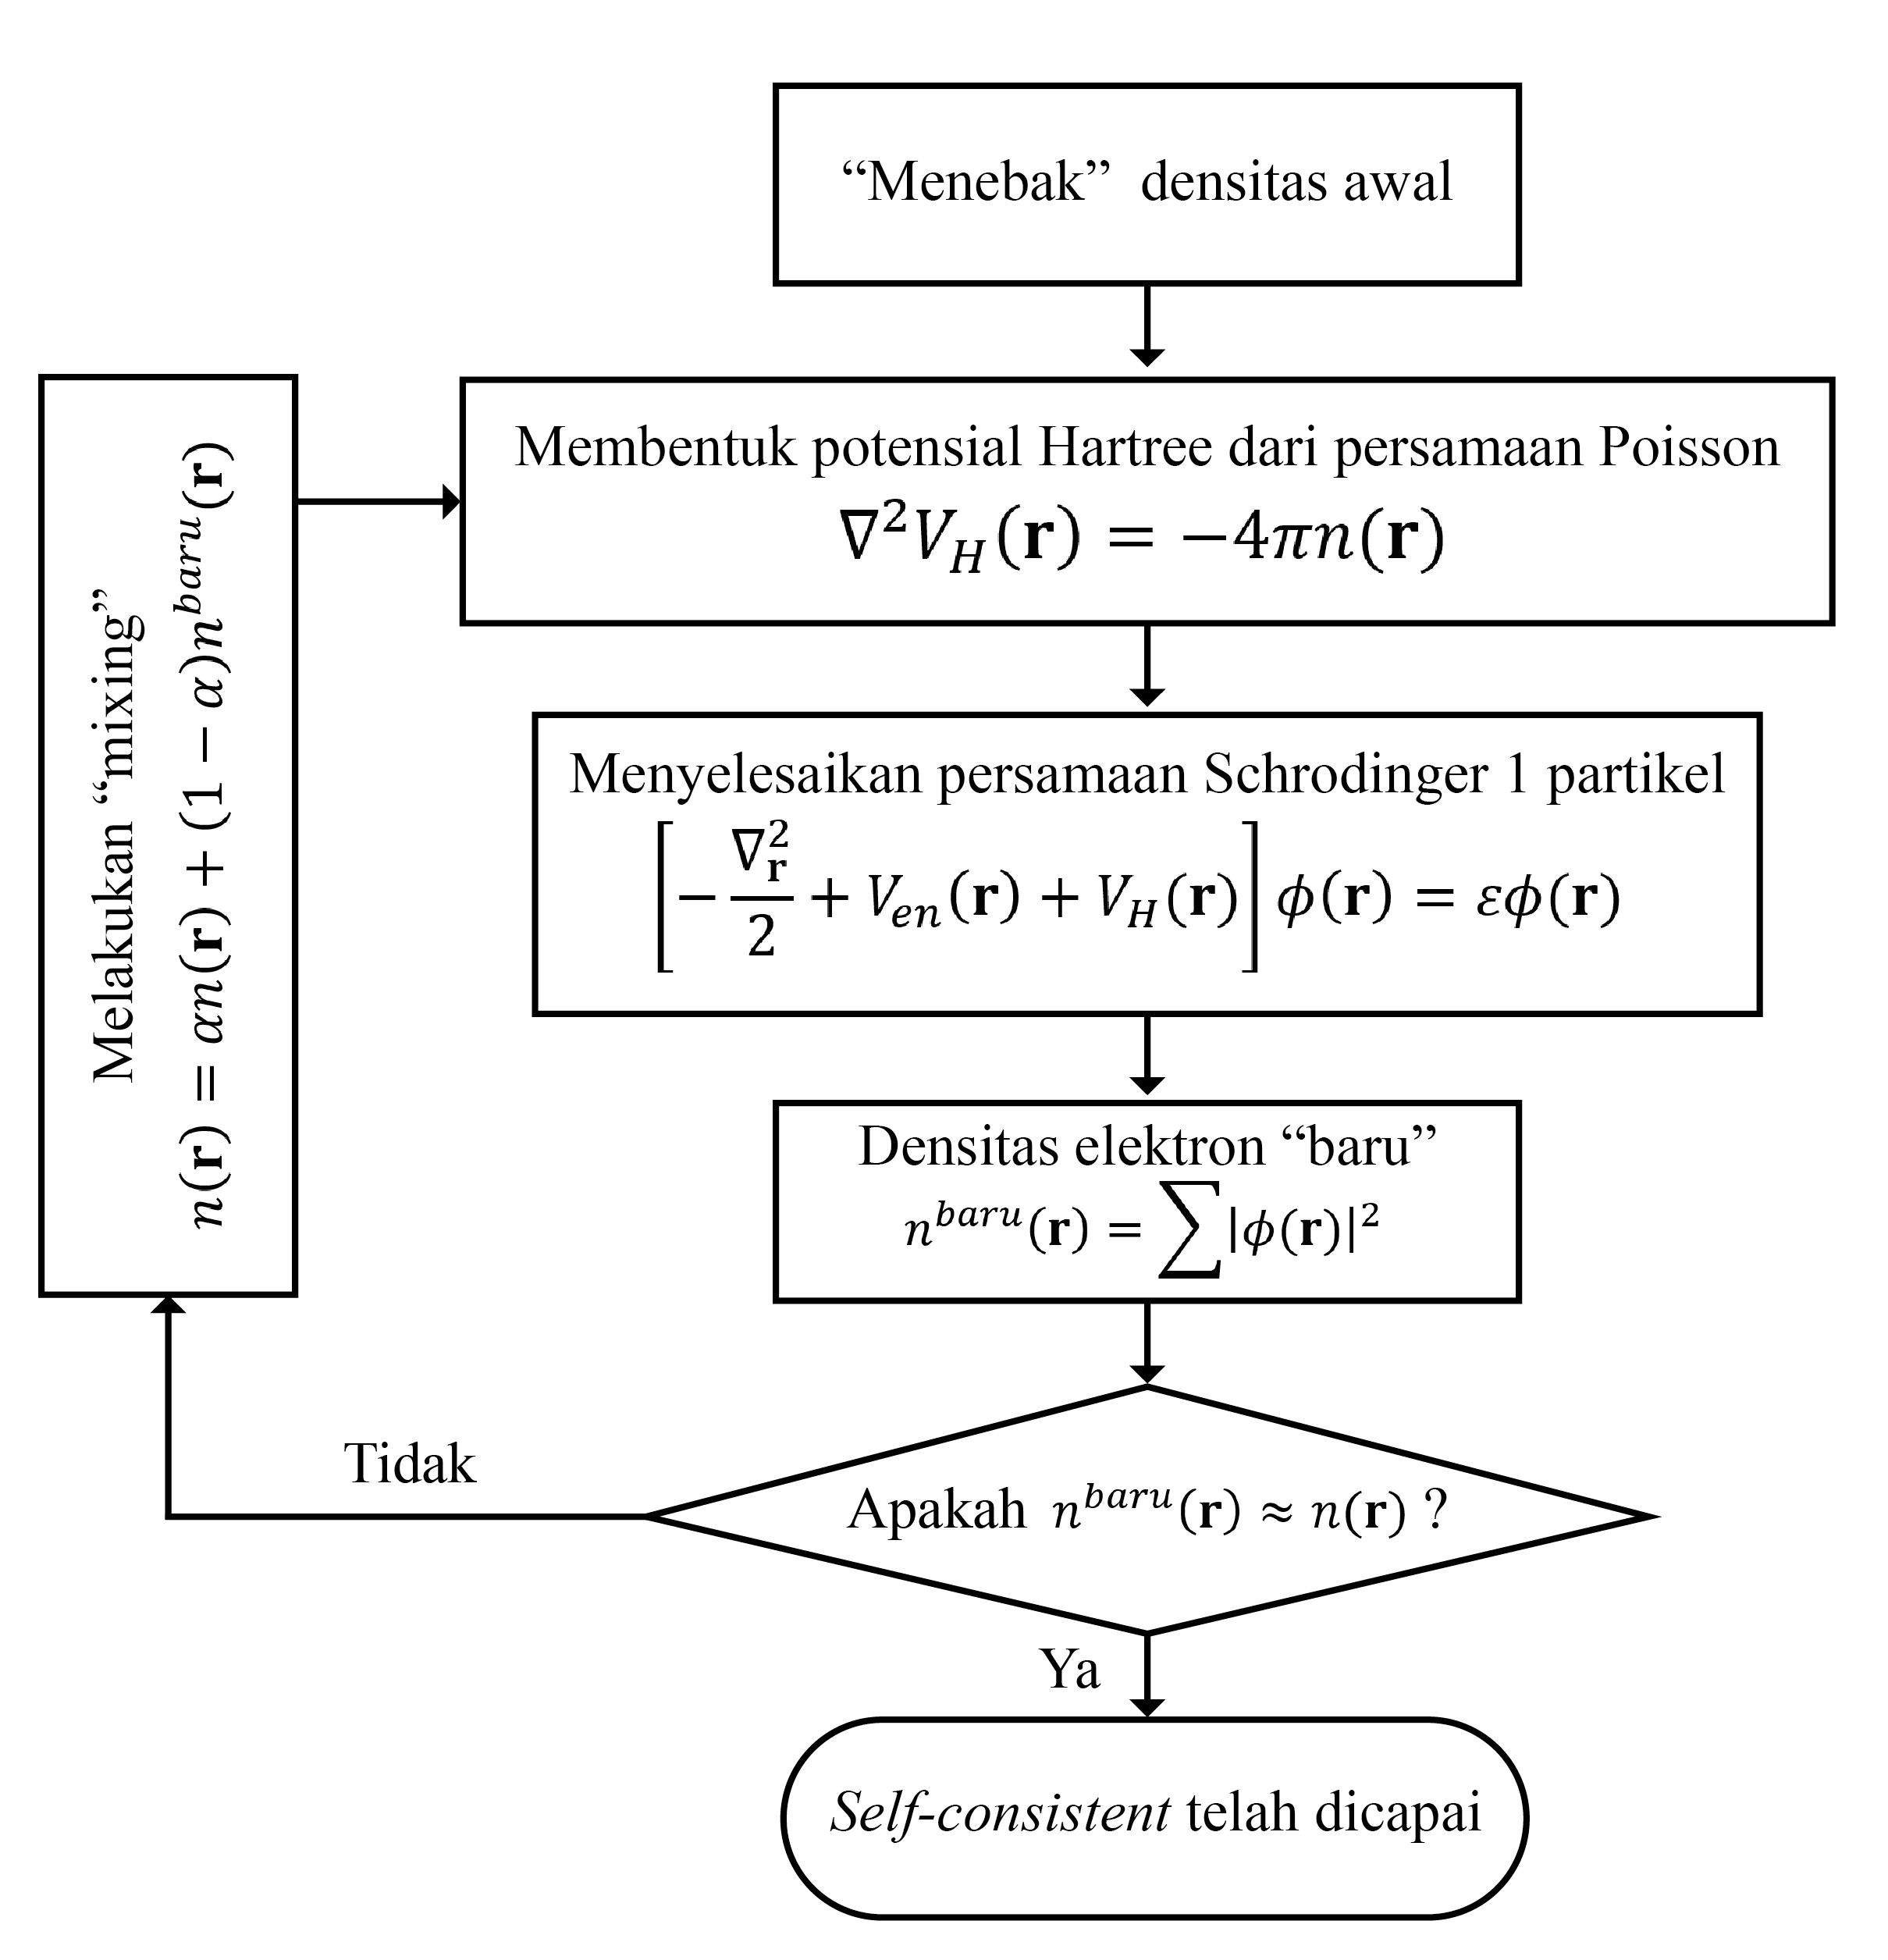
\includegraphics[width=12cm]{gambar/Flowchart SCF.png}
    \caption{Siklus kalkulasi \textit{self-consistent field}.}
    \label{fig:SCF}
\end{figure}
Prinsip perhitungan nilai energi yang digunakan ialah dengan skema \texttt{scf}. Skema ini dapat dilihat pada Gambar \ref{fig:SCF} Perhitungan dilakukan dengan memberikan potensial inti yang dikonstruksi, dimana dalam Quantum ESPRESSO potensial ini ditentukan oleh \textit{pseudopotential} yang didapatkan dari \textit{library} Quantum ESPRESSO. Tebakan awal dari kerapatan berasal dari atom-atom yang digunakan, yang selanjutnya akan digunakan untuk menghitung potensial Hartree dan potensial \textit{exchange-correlation}. Potensial efektif merupakan gabungan antara potensial inti, Hartree dan \textit{exchange-correlation} yang dimasukan di dalam persamaan Kohn-Sham. \textit{Output} dari persamaan menjadi \textit{input} dakam iterasi kembali hingga siklus ini mencapai \textit{self-consistent}. Kondisi \textit{self-consistent} ini terjadi saat kerapatan elektron hasil persamaan Khon-Sham dengan nilai kerapatan awal. Nilai kerapatan ini merupakan kerapatan pada kondisi \textit{ground-state} untuk mendapatkan energi sesuai dengan teorema Hohenberg-Kohn, namun jika \textit{self-consistent} tidak tercapai maka perlu dilakukan konstruksi fungsi kerapatan yang baru dan dilakukan iterasi kembali.

Perhitungan \texttt{scf} akan terus dilakukan hingga sistem berada pada keadaan yang paling stabil, yaitu keadaan dengan nilai energi terendah. Setelah file input dijalankan dengan perintah,
\begin{lstlisting}
    mpirun -np 6 pw.x  < vc-relax.in > vc-relax.out
\end{lstlisting}
akan diperoleh file output graphene.relax.out yang menginformasikan koordinat atom dan parameter kisi yang sudah teroptimalisasi seperti berikut

\begin{lstlisting}
    Begin final coordinates
     new unit-cell volume =   2563.91358 a.u.^3 (   379.93279 Ang^3 )
     density =      1.03767 g/cm^3

CELL_PARAMETERS (alat=  8.84391826)
   1.000753744   0.000000000   0.000000000
  -0.500376872   0.866678165   0.000000000
   0.000000000   0.000000000   4.273504274

ATOMIC_POSITIONS (crystal)
Sn            0.3333333330        0.6666666660        0.5000000000    
Sn            0.6666666660        0.3333333330        0.4579351681
\end{lstlisting}
output di atas merupakan koordinat optimal dari stanene yang digunakan dalam penelitian ini. Terlihat bahwa kita diberikan dua parameter yaitu \texttt{CELL\_PARAMETERS}, dan \texttt{ATOMIC\_POSITIONS}. Nilai inilah yang akan kita gunakan untuk melakukan perhitungan lanjut seperti struktur pita dan rapat keadaan. Perlu diingat bahwa secara praktis kita tidak perlu memasukkan \texttt{CELL\_PARAMETERS} ketika kita mendefinisikan \texttt{ibrav} = 4.

\subsubsection{Perhitungan Struktur Pita}
Perhitungan struktur pita dilakukan dengan 3 file input, yang pertama adalah file input kalkulasi \texttt{scf}, kedua adalah kalkulasi \texttt{bands}, dan terakhir adalah file input untuk mengekstrak data struktur pita. File input \texttt{scf} pada perhitungan struktur pita sama dengan file input \texttt{scf} sebelumnya, namun pada \texttt{name card} \texttt{SYSTEM} perlu ditambah \textit{name list} \texttt{nbnd} yang mana namelist ini diperlukan untuk visualisasi jumlah keadaan yang ingin ditinjau.
\begin{lstlisting}
nbnd    = 16
\end{lstlisting}
kemudiaan file input \texttt{scf} dapat dijalankan dengan perintah
\begin{lstlisting}
mpirun -np 6 pw.x  < scf.in > scf.out
\end{lstlisting}

File kedua yaitu file yang serupa dengan file \texttt{scf} namun kita hanya mengganti \texttt{calculation} menjadi \texttt{'bands'}, dan mendefinisikan \texttt{K\_POINTS} secara lebih spesifik. Jika sebelumnya \texttt{K\_POINTS} mendefinisikan berapa jumlah grid untuk membagi daerah Brilloiun, di kalkulasi \texttt{bands} kita mendefinisikan \texttt{K\_POINTS} menjadi koordinat titik-titik \textit{high-symmetry point} seperti berikut.
\begin{lstlisting}
K_POINTS (crystal_b)
 4
 gG 40
 K 20
 M 30
 gG 0
\end{lstlisting}
dalam input di atas, jalur (\textit{k-path}) yang kita tentukan dari berawal titik $\Gamma$, K, M, dan $\Gamma$. Angka-angka di samping koordinat \textit{high-symmetry point} adalah perintah untuk membagi jalur (k-path) menjadi beberapa titik. Misal pada titik $\Gamma$ ke titik K, kita membagi jalur ini menjadi 50 titik yang akan dihitung dalam kalkulasi \texttt{bands}.

Langkah terakhir adalah mengekstraksi data perhitungan \texttt{bands} dari kalkulasi sebelumnya. Kita siapkan file input sebagai berikut
\begin{lstlisting}
&BANDS
 outdir  = '../tmp/'
 prefix  = 'stanene'
 filband = 'stanene.bands'
/

\end{lstlisting}
kemudian input ini dijalankan dengan perintah
\begin{lstlisting}
mpirun -np 6 bands.x < bands.in > bands.out
\end{lstlisting}
setelah \texttt{JOB DONE}, kita akan memperoleh file dengan format '.gnu'. File tersebut berisi dua kolom yang masing-masing memberikan nilai energi dan koordinat energi  tersebut dalam ruang vektor. File tersebut bisa lansung di-\textit{plot} menggunakan matplotlib.

\subsubsection{Perhitungan Rapat Keadaan (\textit{Density of States})}
Sama seperti perhitungan struktur pita, dalam perhitungan rapat keadaan, kita juga perlu file input \texttt{scf}. Namun 2 hal yang berbeda di sini adalah file kalkulasi '\texttt{nscf}' dan file input ekstraksi data-nya. Sebelumnya, dalam perhitungan \texttt{scf}, fungsi gelombang Kohn-Sham dan densitas elektron diterapkan untuk mencapai kondisi kesetimbangan, di mana potensial efektif dan densitas konvergen. Namun, hasil \texttt{scf} hanya memberikan informasi tentang struktur dasar elektronik dari sistem.

Perhitungan \texttt{nscf} dilakukan dengan mempertahankan struktur geometri dan densitas elektron yang telah dihasilkan dari perhitungan \texttt{scf}, tetapi mengubah beberapa parameter, seperti jumlah \texttt{K-POINTS} atau mesh dalam ruang k (\textit{k-space}), dan mendapatkan spektrum energi lebih lengkap di sekitar titik-titik tertentu di dalam zona Brillouin. Jadi misalnya di \texttt{scf} sudah diperoleh fungsi gelombang, maka di \texttt{nscf} akan diiterasi dengan interpolasi yang lebih rapat. File input \texttt{nscf} persis sama dengan \texttt{scf}, hanya saja kita merubah bagian \texttt{calculation} menjadi \texttt{'nscf'} seperti berikut.
\begin{lstlisting}
calculation = 'nscf'
\end{lstlisting}
kemudian pada \textit{name cards} \texttt{CONTROL} ditambahkan \texttt{verbosity = 'high'}, dan pada \texttt{SYSTEM} ditambahkan \texttt{"occupation = tetrahedra"}. Jenis \texttt{occupation} yang kita pilih berpengaruh pada bentuk rapat keadaan yang dihasilkan.
Berdasarkan penelitian sebelumnya \citep{toriyama2021comparison}, diketahui bahwa occupation jenis tetrahedra memberikan data yang lebih akurat untuk perhitungan rapat keadaan dibanding jenis \texttt{occupation} lain, seperti \texttt{gaussian}.

File ekstraksi data dos adalah
\begin{lstlisting}
&DOS
outdir = '../tmp'
prefix = 'stanene'
fildos = 'stanene.dos'
/
\end{lstlisting}
berbeda dengan \texttt{bands} output dari perhitungan \texttt{dos} adalah file dengan format '.dos' file ini berupa data dos yang siap di-\textit{plot} menggunakan matplotlib.
    %%%%%%%%%%%%%%%%%%%%%%%%%%%%%%%%%%%%%%%%%%%%%%%%%%%%%%%%%%%%%%%%%%%%%%
%%%%%%%%%%%%%%%%%%%%%%%%%%%%%%%%%%%%%%%%%%%%%%%%%%%%%%%%%%%%%%%%%%%%%%
% BAB HASIL DAN PEMBAHASAN:
%=====================================================================
\renewcommand{\thechapter}{\Roman{chapter}}
\addtocontents{toc}{\vskip10pt}
\chapter{HASIL DAN PEMBAHASAN}
\renewcommand{\thechapter}{\arabic{chapter}}
%---------------------------------------------------------------------

%=====================================================================
\section{Pra-Kalkulasi Sifat Elektronik}
%=====================================================================
Sebelum dilakukannya proses kalkulasi untuk struktur pita dan rapat keadaan, kita harus memastikan bahwa parameter-parameter yang kita gunakan sudah sesuai dan efisien dari segi waktu dan biaya komputasi. Salah satu parameter penting dalam input perhitungan DFT kami ialah \textit{cutoff} energi kinetik dan K-POINTS. Kedua parameter ini perlu diselidiki kekonvergenannya. Selain itu struktur yang digunakan harus dalam konfigurasi dengan tingkat energi paling rendah (stabil). Dalam pra-kalkulasi di bawah akan ditentukan parameter \texttt{ecutwfc}, \texttt{K-POINTS}, dan optimasi struktur \texttt{vc-relax}.\nocite{Giannozzi_2017}\nocite{giannozzi2020quantum}

%=====================================================================
\subsection{Konvergensi \textit{cutoff} Energi Kinetik (\texttt{ecutwfc})}
%=====================================================================
Salah satu input terpenting dalam Quantum ESPRESSO \textit{cutoff} adalah energi kinetik. Dalam Quantum ESPRESSO, fungsi gelombang elektron diaproksimasi dalam basis gelombang datar \textit{(plane wave basis)}\citep{DFTSholl}. \textit{Cutoff} Energi kinetik menentukan jumlah maksimum gelombang datar yang digunakan dalam perhitungan. Semakin tinggi \textit{cutoff} energi kinetik, semakin banyak gelombang datar yang digunakan, yang dapat meningkatkan presisi perhitungan. Namun, peningkatan ini juga akan meningkatkan kompleksitas dan waktu komputasi. Pemilihan \textit{cutoff} energi kinetik harus mempertimbangkan keseimbangan antara kepresisian hasil yang diinginkan dan biaya komputasi yang dapat diterima. Jika \textit{cutoff} energi kinetik terlalu rendah, hasil perhitungan dapat menjadi tidak akurat. Di sisi lain, jika \textit{cutoff} energi kinetik terlalu tinggi, waktu komputasi dapat menjadi lebih lama dan tidak efisien. Dalam sistem periodik, fungsi gelombang bidang dieksoresikan sebagai \citep{Giannozzi_2009}
\begin{equation}
    \psi (\textbf{r}) = \frac{1}{\Omega} \sum_\textbf{G} c_{\textbf{k},\textbf{G}} e^{i(\textbf{k}+\textbf{G})\cdot\textbf{r}}
\end{equation}
di mana \textbf{G} adalah vektor kisi resiprok. Gelombang bidang ini dapat direpresentasikan sebagai sebuah \textit{grid} (kisi) dalam bidang-k (\textit{k-plane}). Semakin banyak grid yang kita gunakan, akan semakin akurat hasil kalkulasi yang kita jalankan, namun akan menambah biaya dan efisiensi kalkulasi. Secara prinisp, jumlah gelombang bidang yang memenuhi perioditas material adalah tak hingga dan tidak mungkin bagi kita menghitung gelombang bidang sebanyak itu. Oleh karena itu kita harus membatasi jumlah gelombang bidang yang akan kita hitung dengan cara membatasi panjang gelombang minimum $\lambda_{min}$ dalam ruang vektor. Penentuan panjang panjang gelombang minimun berkorespondensi terhadap bentuk maksimum vektor gelombang pada ruang vektor sebagai berikut,
\begin{equation}
    |\textbf{G}_{max}|= \frac{2\pi}{\lambda_{min}}
\end{equation}
Kemudian dari persamaan (4.2) dapat dibentuk definisi dari \textit{cutoff} energi kinetik sebagai berikut
\begin{equation}
    E_{cut}=\frac{\hbar^2}{2m} |\textbf{G}_{max}|
\end{equation}
dan kita membatasi \textit{cutoff} energi dengan batasan sebagai berikut
\begin{equation}
    \frac{\hbar|\textbf{k}+\textbf{G}|}{2m}\le E_{cut}
\end{equation}
jadi dengan menentukan \textit{cutoff} energi kinetik secara tidak lansung kita menentukan panjang gelombang minimum pada ruang vektor yang berkorespondensi dengan jumlah gelombang bidang yang akan kita gunakan dalam kalkulasi.

Dalam penelitian ini, dilakukan perhitungan SCF dengan beberapa variasi \texttt{ecutwfc}. seperti yang terlihat pada gambar 4.1 energi total mulai konvergen ketika \texttt{ecutwfc} bernilai 30 Rydberg jadi untuk kepresisian dan efisiensi kalkulasi, penulis menggunakan \texttt{ecutwfc} sebesar 60 Rydberg. nilai \texttt{ecutwfc} diambil karena merupakan saran dari sumber \textit{pseudopotential} SSSP Materials Cloud. Sedangkan untuk input \texttt{ecutrho} penulis menggunakan nilai \textit{default} 480 Rydberg \texttt{ecutwfc} dengan saran dari sumber \textit{pseudopotential} yang sama.

\begin{figure}
    \centering
    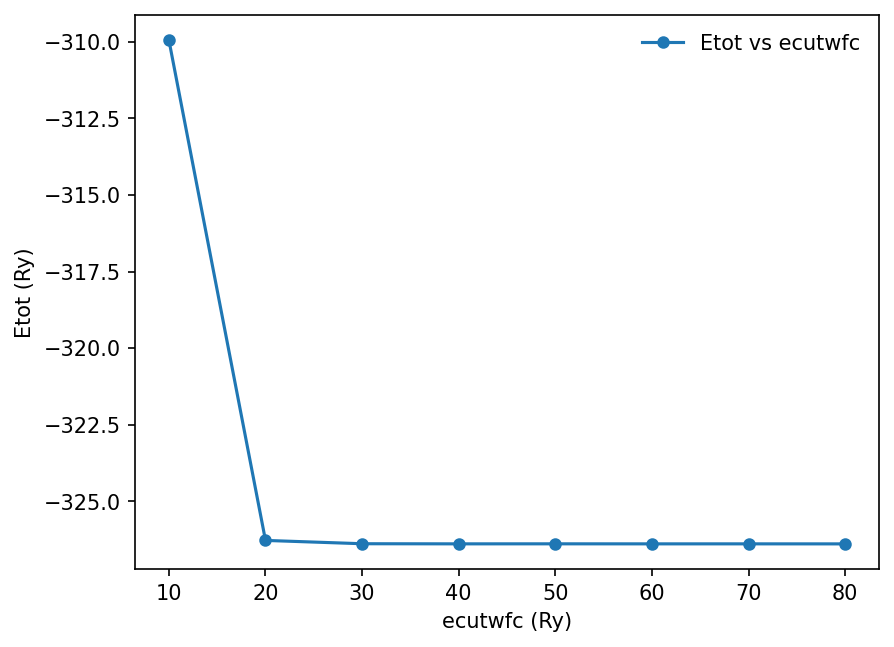
\includegraphics[width=15cm]{./gambar/plot_ecut_sn.png}
    \caption{Konvergensi \textit{cutoff} energi kinetik}
    \label{fig:ecutwfc}
\end{figure}



%-------------------------------------------------------------------


%=====================================================================
\subsection{Konvergensi \texttt{K-POINT}}
%=====================================================================
\texttt{K-POINT} mengacu pada titik-titik dalam ruang momentum yang digunakan dalam perhitungan untuk merepresentasikan distribusi elektron dalam struktur kristal. Sama halnya dengan \texttt{ecutwfc} Pemilihan \texttt{K-POINTS} mempengaruhi akurasi dan kecepatan perhitungan.
\begin{figure}
    \centering
    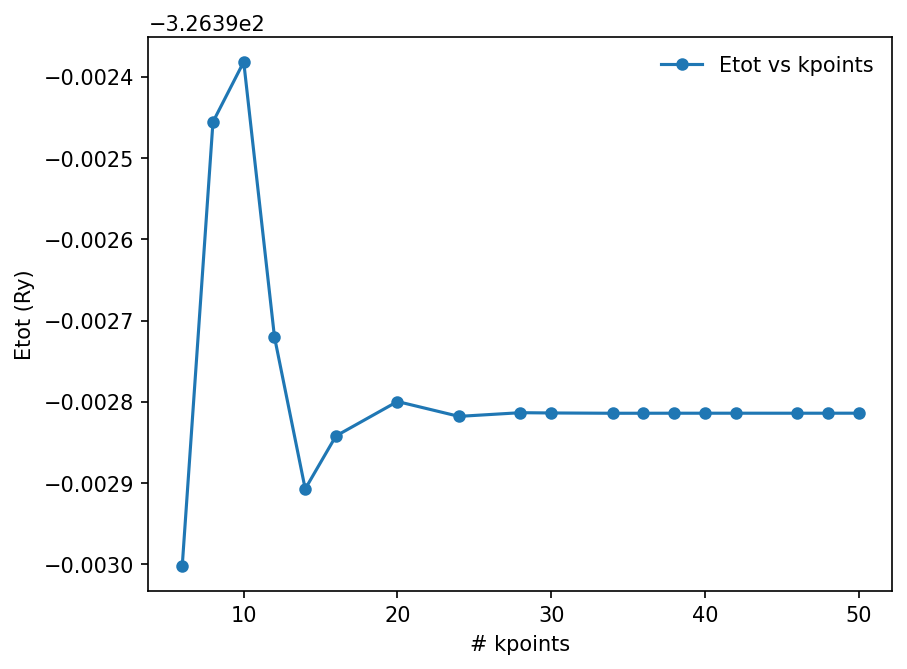
\includegraphics[width=15cm]{./gambar/plot_kpoints_sn.png}
    \caption{Konvergensi K-points}
    \label{fig:kpoints}
\end{figure}
Dalam metode DFT yang digunakan oleh Quantum ESPRESSO, distribusi elektron dalam struktur kristal diwakili oleh fungsi gelombang Bloch. Fungsi gelombang ini diekspansi dalam basis gelombang datar (\textit{plane wave basis}) dan faktor fase Bloch. Titik-titik k dalam ruang momentum menentukan faktor fase Bloch dan mewakili kontribusi dari setiap bagian dalam \textit{Brillouin Zone} (BZ). Dalam penelitian kali ini, nilai energi total mulai konvergen pada variasi \texttt{K\_POINT} $18\times18\times1$. Namun, untuk meningkatkan akurasi, penulis menggunakan variasi $24\times24\times1$ untuk struktur \textit{stanene}

\subsection{Optimasi Struktur (\texttt{vc-relax})}
Optimasi struktur input kita dilakukan melalui perhitungan Perhitungan \texttt{vc-relax} dalam Quantum ESPRESSO adalah perhitungan yang digunakan untuk mengoptimalkan struktur kristal dalam keadaan yang rileks secara volumetrik dan sel yang rileks. "vc" dalam \texttt{vc-relax} adalah singkatan dari \textit{volume and cell}, yang menunjukkan bahwa perhitungan ini memperhatikan optimisasi volume dan sel.
\begin{figure}
    \centering
    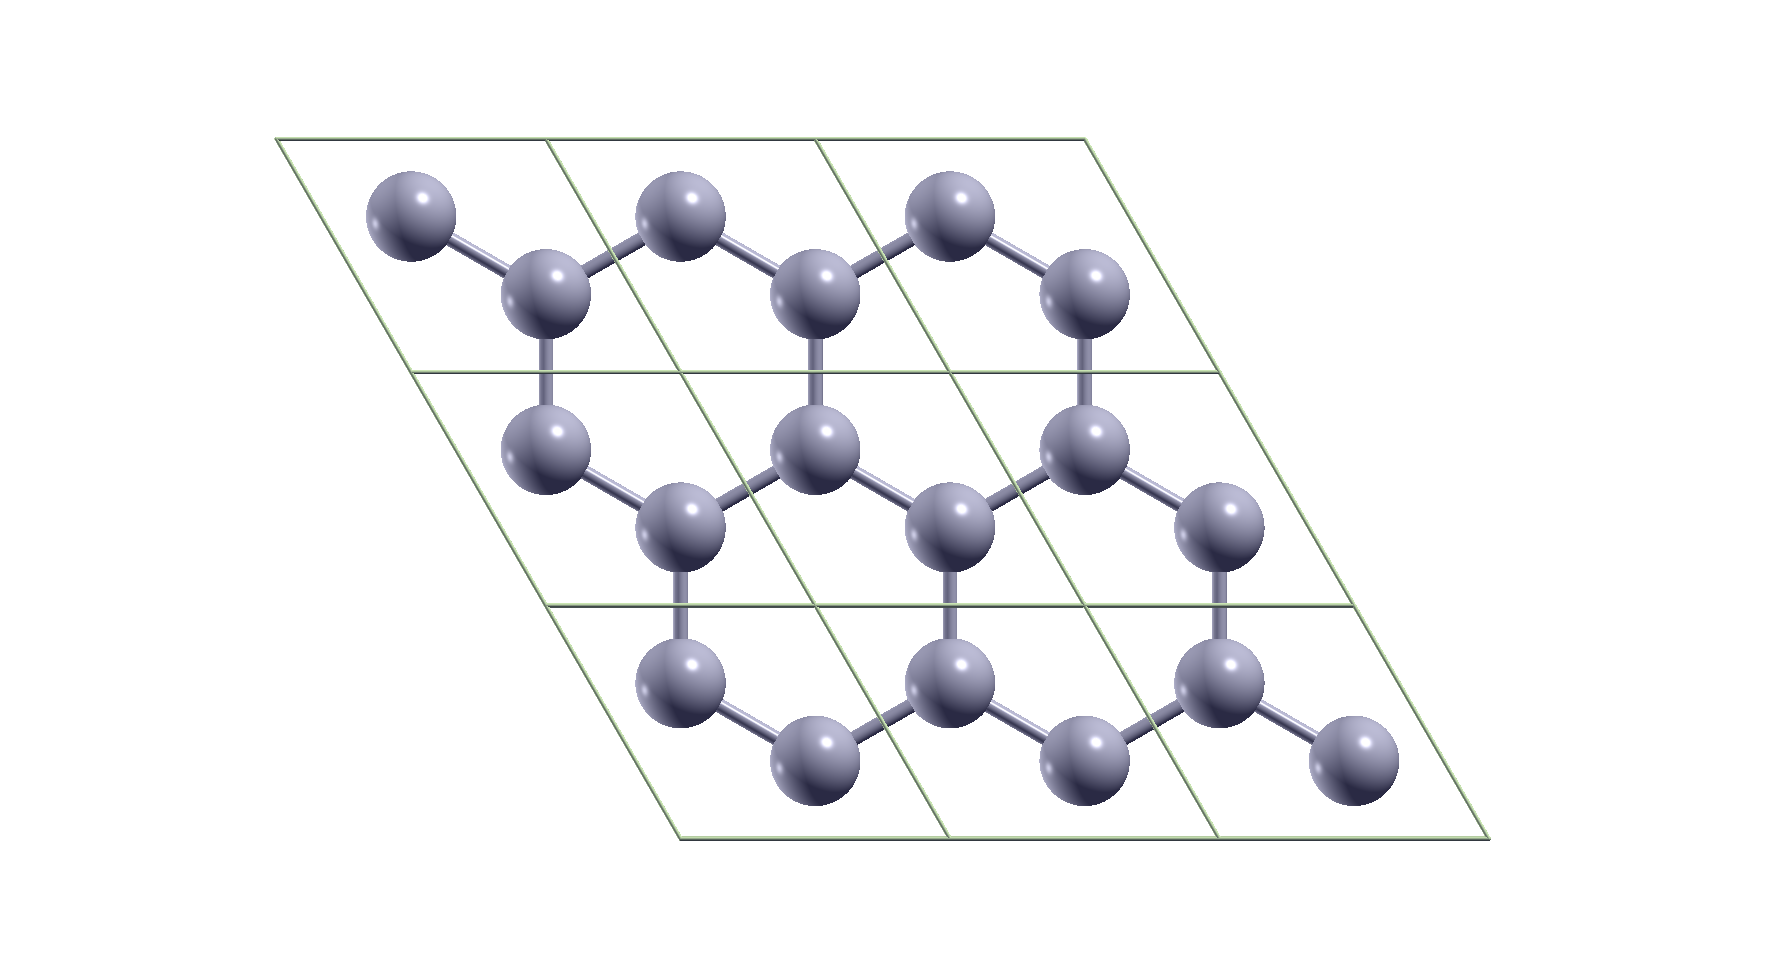
\includegraphics[width=15cm]{./gambar/pw.vc-relax.sn.png}
    \caption{Struktur optimal dari stanene}
    \label{fig:DensityofStates}
\end{figure}
Tujuan utama perhitungan \texttt{vc-relax} adalah menemukan struktur kristal yang memiliki minimum energi total dengan memvariasikan volume sel serta parameter sel seperti vektor basis. Proses optimisasi dilakukan dengan mengubah parameter-parameter ini dan menghitung ulang distribusi elektron dan energi total menggunakan metode DFT. Selama perhitungan \texttt{vc-relax}, Quantum ESPRESSO akan menyesuaikan volume sel dan parameter sel untuk mencapai keseimbangan energi minimum. Selain itu, distribusi elektron dalam struktur kristal juga akan disesuaikan untuk mencapai konvergensi yang baik. Sesuatu yang akan kita perleh dari perhtiungan ini adalah informasi penting tentang struktur kristal seperti konstanta kisi dan parameter sel optimal. Nilai optimal yang kita peroleh akan kita gunakan untuk perhitungan selanjutnya seperti mencari struktur pita maupun rapat keadaan.

Perhitungan \texttt{vc-relax} yang kami jalankan memungkinkan atom bergerak dalam arah $x$ dan $y$ saja. Perhitungan ini dapat diatur pada bagian "\texttt{cell dofree}". Setelah kalkulasi \texttt{vc-relax} dilaksanakan maka diperoleh struktur optimal untuk parameter konstanta kisi sebesar 4.68 \AA. Nilai yang kami peroleh sesuai dengan penelitian-penelitian sebelumnya. Gambar 4.3 menunjukan bentuk struktur optimal untuk Stanene


\section{Kalkulasi Sifat Elektronik}
Dalam menghitung struktur elektronik dari material stanene diperoleh struktur pita energi atau band structure dan rapat keadaan total atau density of state (rapat keadaan). Struktur pita elektronik merupakan kurva energi terhadap bilangan gelombang yang menunjukkan rentang energi yang diperbolehkan serta yang tidak diperbolehkan adanya fungsi gelombang elektron [Kittel, 2005]. Untuk mengetahui sifat material dapat diketahui dengan melihat letak potensial kimia berada dan seberapa besar \textit{band gap} yang dimiliki material. Setelah struktur optimal diperoleh maka dapat diperoleh struktur pita dan
rapat keadaan dari stanene. K-path pada zona brilloin yang digunakan adalah
Γ – K – M - Γ.

\subsection{Struktur Elektronik Stanene}
Dalam studi ini dibentuk kembali struktur pita energi dan rapat keadaan dari stanene . Hasil dari simulasi kami menunjukkan struktur pita energi stanene yang konsisten dengan penelitian sebelumnya. 

\begin{figure}[h]

\begin{subfigure}{0.5\textwidth}
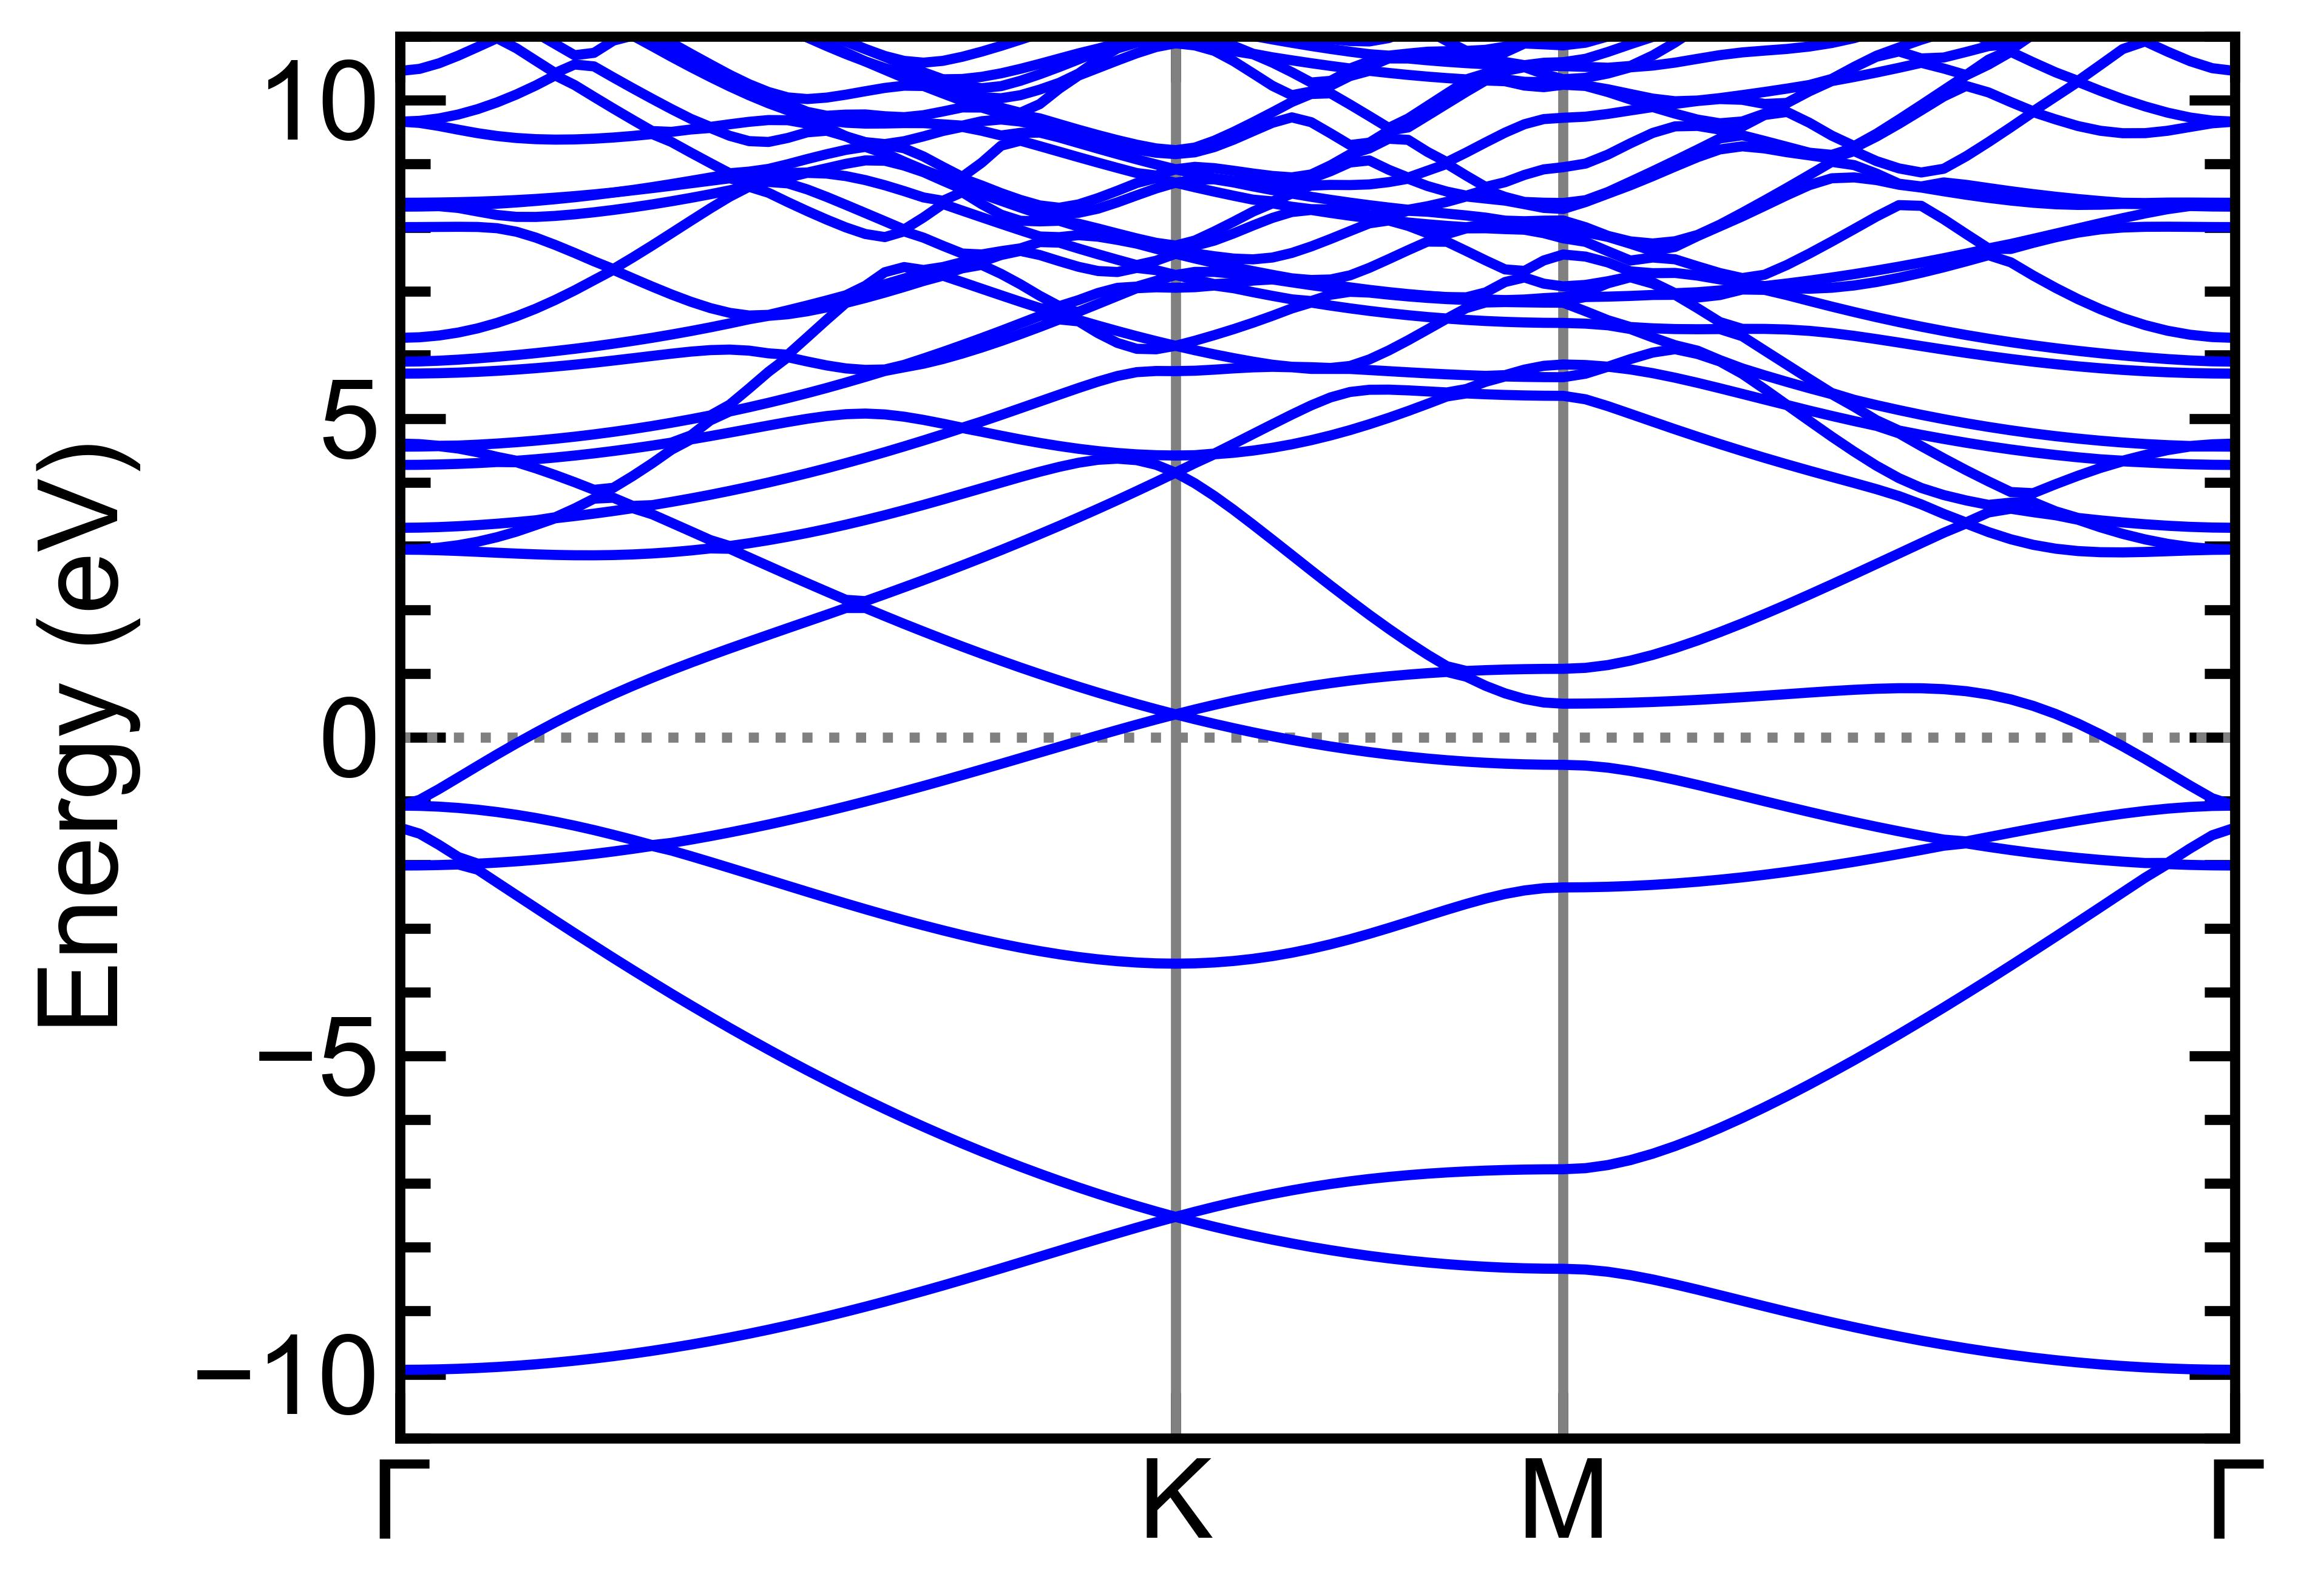
\includegraphics[width=0.9\linewidth, height=6cm]{gambar/plot_sn_bands.jpg} 
\caption{bands structure}
\label{fig:subim1}
\end{subfigure}
\begin{subfigure}{0.5\textwidth}
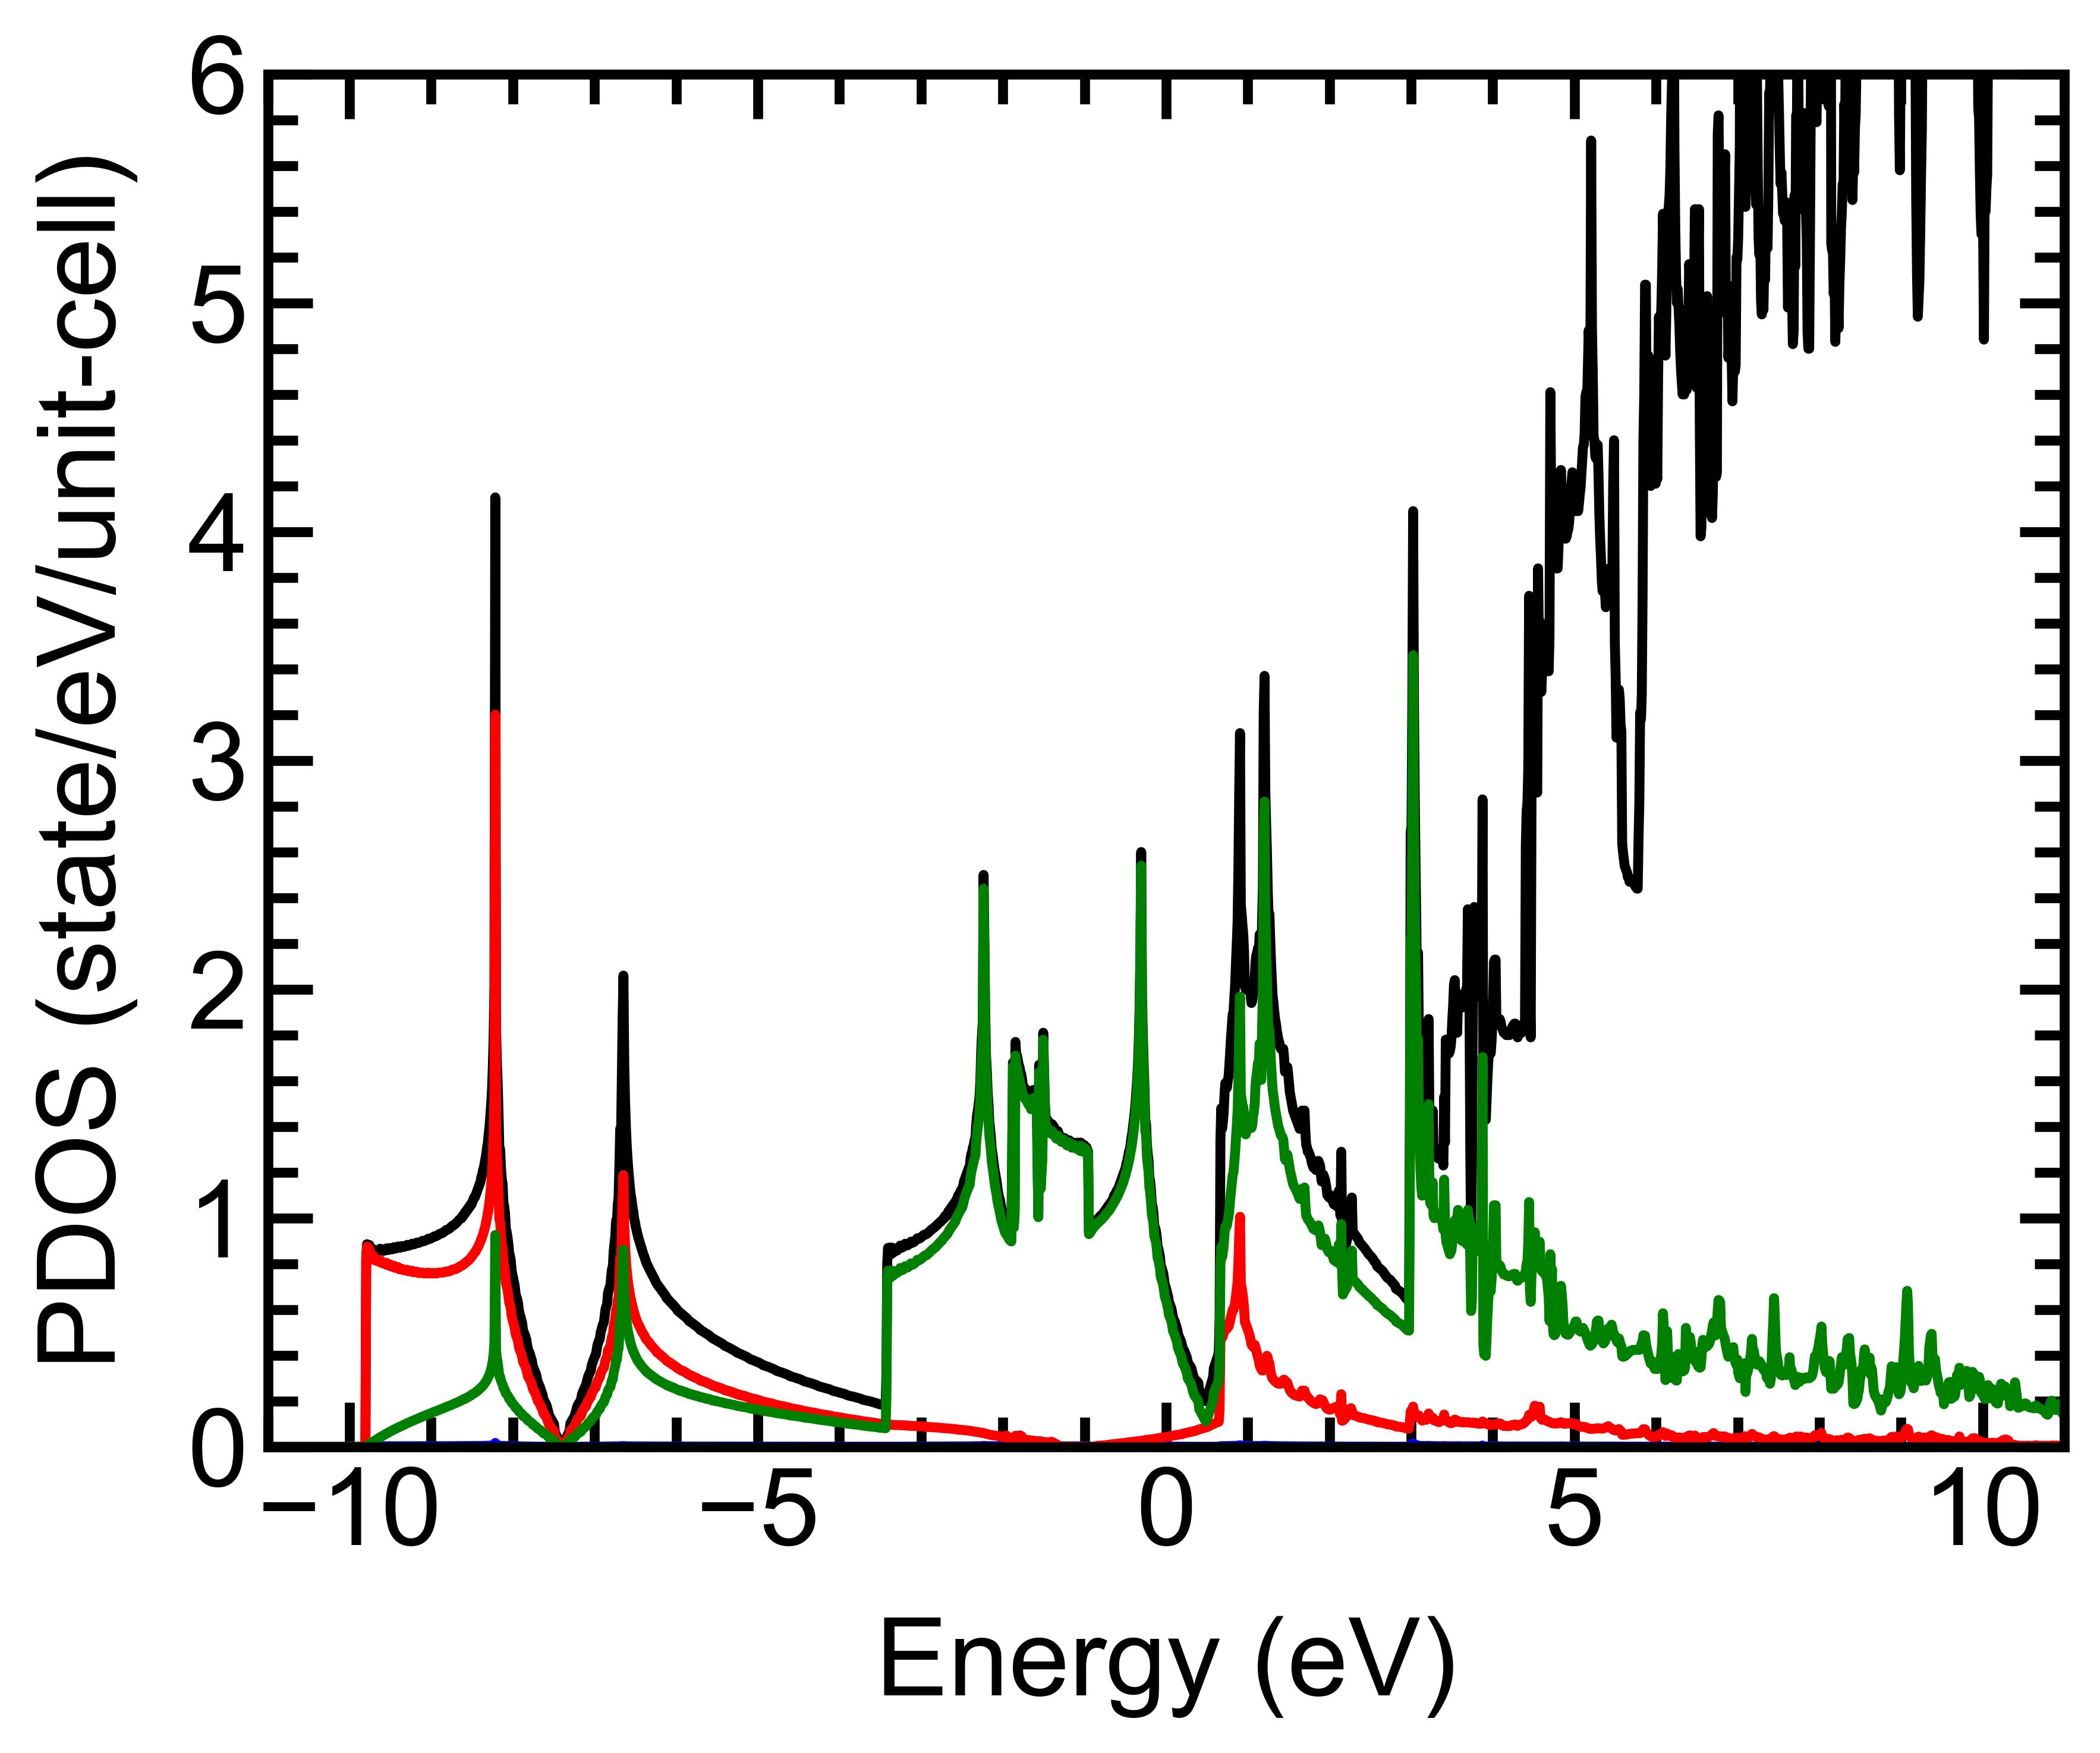
\includegraphics[width=0.9\linewidth, height=6cm]{gambar/graph_sn_pdos.jpg}
\caption{DOS dengan garis hijau adalah orbital s dan garis merah adalah orbital p}
\label{fig:subim2}
\end{subfigure}

\caption{sifat elektronik dasar dari stanene}
\label{fig:dos dan bands sn}
\end{figure}

\begin{figure}[h]
\centering
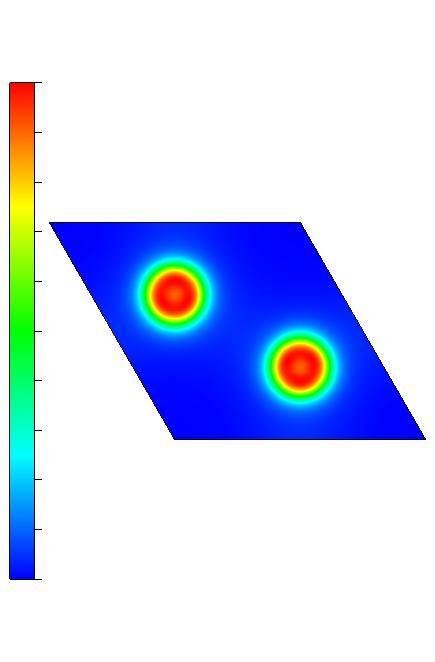
\includegraphics[width=0.5\linewidth]{gambar/sn_rho.jpg}
\caption{Rapat muatan dari stanene}
\label{fig:charge density}
\end{figure}

Seperti yang terlihat pada Gambar \ref{fig:dos dan bands sn} pita energi stanene menunjukkan dua dispersi pita, yaitu pita valensi dan pita konduksi. Pita valensi berada di bawah energi Fermi, sementara pita konduksi berada di atasnya. Selain itu, pita valensi dan konduksi saling berdekatan di titik K menunjukkan adanya tumpang tindih antara pita-pita ini yang membuat titik K memiliki Dirac cone. Fenomena Dirac cone pada titik K di stanene menurut \citep{C6RA26169H} terdiri dari orbital $5P_z$ yang menjamin stabilitas stanene dalam membentuk ikatan-$\pi$

Sementara itu rapat keadaan yang disajikan dalam grafik mengacu pada jumlah keadaan energi yang tersedia untuk elektron dalam bahan atau zat padat pada setiap tingkat energi. Ini memberikan gambaran tentang distribusi energi elektron dalam bahan dan berguna untuk memahami sifat elektronik bahan seperti konduktivitas listrik dan sifat-sifat elektronik lainnya. Rapat keadaan sering diukur dalam satuan keadaan per energi (per unit energi atau per unit massa) dan digunakan untuk menggambarkan perilaku sistem zat padat secara keseluruhan atau pada tingkat lokal.

Jenis occupation dalam file input DOS yang digunakan pada penelitian ini adalah “\texttt{tetrahedra}”. Selain \texttt{tetrahedra}, jenis occupation lain yang umum digunakan adalah \texttt{smearing} yang dibagi lagi menjadi \texttt{gaussian}, \texttt{marzari-vanderbilt}, dan \texttt{fermi-dirac}. Alasan penggunaan “tetrahedra” dalam kalkulasi DOS pada penelitian ini karena \texttt{tetrahedra} menjamin keakuratan yang lebih baik dibandingkan “smearing”. Metode tetrahedra membagi zona Brillouin menjadi tetrahedra, menghitung energi eigen di sudut-sudut setiap tetrahedron, dan secara linear menginterpolasi nilai energi eigen di dalam setiap tetrahedron untuk melakukan integrasi \citep{toriyama2021comparison}.

Pada penelitian ini juga mendapatkan distribusi kerapatan muatan dapat memberikan informasi tentang sifat ikatan antara berbagai atom. Sebagai contoh, jika muatan valensi terlokalisasi di lokasi atom, dan tidak ada muatan di antara atom, atau di ruang antar atom, maka bahan tersebut memiliki ikatan ionik. Di sisi lain, jika ada tumpukan muatan valensi di antara garis yang menghubungkan pasangan atom, maka mereka terikat secara kovalen. Sejumlah besar muatan valensi yang terdelokalisasi merupakan indikasi ikatan logam. Muatan kepadatan sistem dapat dihitung secara efisien dan divisualisasikan menggunakan alat pasca-pemrosesan yang tersedia di QE.
Pada \ref{fig:charge density} kerapatan muatan stanene diplot. Kerapatan menunjukkan hal yang signifikan yaitu berupa delokalisasi elektron yang menggambarkan kemampuan transportasi muatan terbatas.




    %%%%%%%%%%%%%%%%%%%%%%%%%%%%%%%%%%%%%%%%%%%%%%%%%%%%%%%%%%%%%%%%%%%%%%
%%%%%%%%%%%%%%%%%%%%%%%%%%%%%%%%%%%%%%%%%%%%%%%%%%%%%%%%%%%%%%%%%%%%%%
% BAB PENUTUP
%=====================================================================
\renewcommand{\thechapter}{\Roman{chapter}}
\addtocontents{toc}{\vskip10pt}
\chapter{PENUTUP}
\renewcommand{\thechapter}{\arabic{chapter}}
%---------------------------------------------------------------------

%=====================================================================
\section{Kesimpulan}
%=====================================================================

Berdasarkan penelitian yang telah dilakukan, dapat ditarik kesimpulan bahwa stanene bersifat konduktor yang berpusat pada titik \texttt{k-points} K. Perbedaan nilai dari penelitian sebelumnya yang dilakukan oleh \citeauthor{sagar2019} kemungkinan besar disebabkan oleh perbedaan parameter atau kesalahan kalkulasi yang digunakan. Dalam penelitian sebelumnya juga disebutkan bahwa untuk struktur 2-dimensi stanene dilakukan dengan menggunakan fungsional PBE-GGA yang diverifikasi oleh fungsional LDA tetapi pada penelitian ini hanya menggunakan fungsional PBE-GGA

%=====================================================================
\section{Saran}
%=====================================================================
\begin{enumerate}
    \item Untuk penelitian selanjutnya, disarankan menggunakan parameter yang digunakan
    \item Mengecek parameter dengan paper yang telah ada
    \item Mengecek hasil sudah akurat atau belum

\end{enumerate}


    
%---------------------------------------------------------------------
%   DAFTAR PUSTAKA
%---------------------------------------------------------------------

    \addtocontents{toc}{\vskip10pt}
    \renewcommand{\bibname}{DAFTAR PUSTAKA}
    \addcontentsline{toc}{chapter}{DAFTAR PUSTAKA}
    %\bibliographystyle{unsrt} % untuk style dengan nomor
    \bibliographystyle{format-pustaka} % untuk style dengan nama
    \bibliography{pustaka}
    
%---------------------------------------------------------------------
%   APPENDIX
%---------------------------------------------------------------------

    {
    \appendix
    \addtocontents{toc}{\vskip10pt}
    \renewcommand{\chaptername}{LAMPIRAN}
    %%%%%%%%%%%%%%%%%%%%%%%%%%%%%%%%%%%%%%%%%%%%%%%%%%%%%%%%%%%%%%%%%%%%%%
% LAMPIRAN A
%%%%%%%%%%%%%%%%%%%%%%%%%%%%%%%%%%%%%%%%%%%%%%%%%%%%%%%%%%%%%%%%%%%%%%

\chapter{Judul Lampiran}

%---------------------------------------------------------------------


\section{File scf dan bands}
%---------------------------------------------------------------------
\subsection{File Input \texttt{scf} stanene}
\begin{lstlisting}
&control
calculation = 'scf'
prefix='stanene',
pseudo_dir = '../pseudo/',
outdir='../tmp/'
/
&system
ibrav = 4,
a=4.68
c=20,
nat = 2,
ntyp = 1,
ecutwfc = 40.0,
occupations = 'smearing'
smearing = 'm-p'
degauss = 0.02
/
&electrons
mixing_beta = 0.7
conv_thr = 1.0d-6
/
ATOMIC_SPECIES
Sn 118.710 Sn_pbe_v1.uspp.F.UPF
ATOMIC_POSITIONS (crystal)
Sn 0.333333333 0.666666666 0.500000000
Sn 0.666666666 0.333333333 0.500000000
K_POINTS {automatic}
24 24 1 0 0 0

\end{lstlisting}

\subsection{File Input \texttt{bands} stanene}

\begin{lstlisting}
&control
calculation = 'scf'
prefix='stanene',
pseudo_dir = '../pseudo/',
outdir='../tmp/'
verbosity = 'high'
/
&system
ibrav = 4,
a=4.683527522,
c=20,
nat = 2,
ntyp = 1,
ecutwfc = 60.0,
ecutrho = 480, 
occupations = 'smearing'
smearing = 'm-p'
degauss = 0.02
/
&electrons
mixing_beta = 0.7
conv_thr = 1.0d-7
/
ATOMIC_SPECIES
Sn 118.710 Sn_pbe_v1.uspp.F.UPF
ATOMIC_POSITIONS (crystal)
Sn            0.3333333330        0.6666666660        0.5000000000
Sn            0.6666666660        0.3333333330        0.5000000000
K_POINTS (automatic)
24 24 1 0 0 0

\end{lstlisting}

\subsection{File Input \texttt{nscf} stanene}
\begin{lstlisting}
&control
calculation = 'nscf'
prefix='stanene',
pseudo_dir = '../pseudo/',
outdir='../tmp/'
verbosity = 'high'
/
&system
ibrav = 4,
a=4.683527522,
c=20,
nat = 2,
ntyp = 1,
ecutwfc = 60.0,
ecutrho = 480, 
occupations = 'tetrahedra'
nbnd = 60
/
&electrons
mixing_beta = 0.7
conv_thr = 1.0d-7
/
ATOMIC_SPECIES
Sn 118.710 Sn_pbe_v1.uspp.F.UPF
ATOMIC_POSITIONS (crystal)
Sn            0.3333333330        0.6666666660        0.5000000000
Sn            0.6666666660        0.3333333330        0.5000000000
K_POINTS (automatic)
60 60 1 0 0 0

\end{lstlisting}





%%%%%%%%%%%%%%%%%%%%%%%%%%%%%%%%%%%%%%%%%%%%%%%%%%%%%%%%%%%%%%%%%%%%%%
    %\input{./halaman-belakang/lampiran/lampiranB}
    }
%---------------------------------------------------------------------
%   BIOGRAFI PENULIS
%---------------------------------------------------------------------

    %%%%%%%%%%%%%%%%%%%%%%%%%%%%%%%%%%%%%%%%%%%%%%%%%%%%%%%%%%%%%%%%%%%%%%
%%%%%%%%%%%%%%%%%%%%%%%%%%%%%%%%%%%%%%%%%%%%%%%%%%%%%%%%%%%%%%%%%%%%%%
% BIOGRAFI PENULIS
%=====================================================================
\renewcommand{\thechapter}{\Roman{chapter}}
\addtocontents{toc}{\vskip10pt}
\chapter*{BIOGRAFI PENULIS}
\renewcommand{\thechapter}{\arabic{chapter}}
%---------------------------------------------------------------------

\begin{wrapfigure}{l}{.35\textwidth}
  \begin{center}
    \vspace{-20pt} % Silahkan disesuaikan apabila space di atas gambar terlalu kecil/besar
    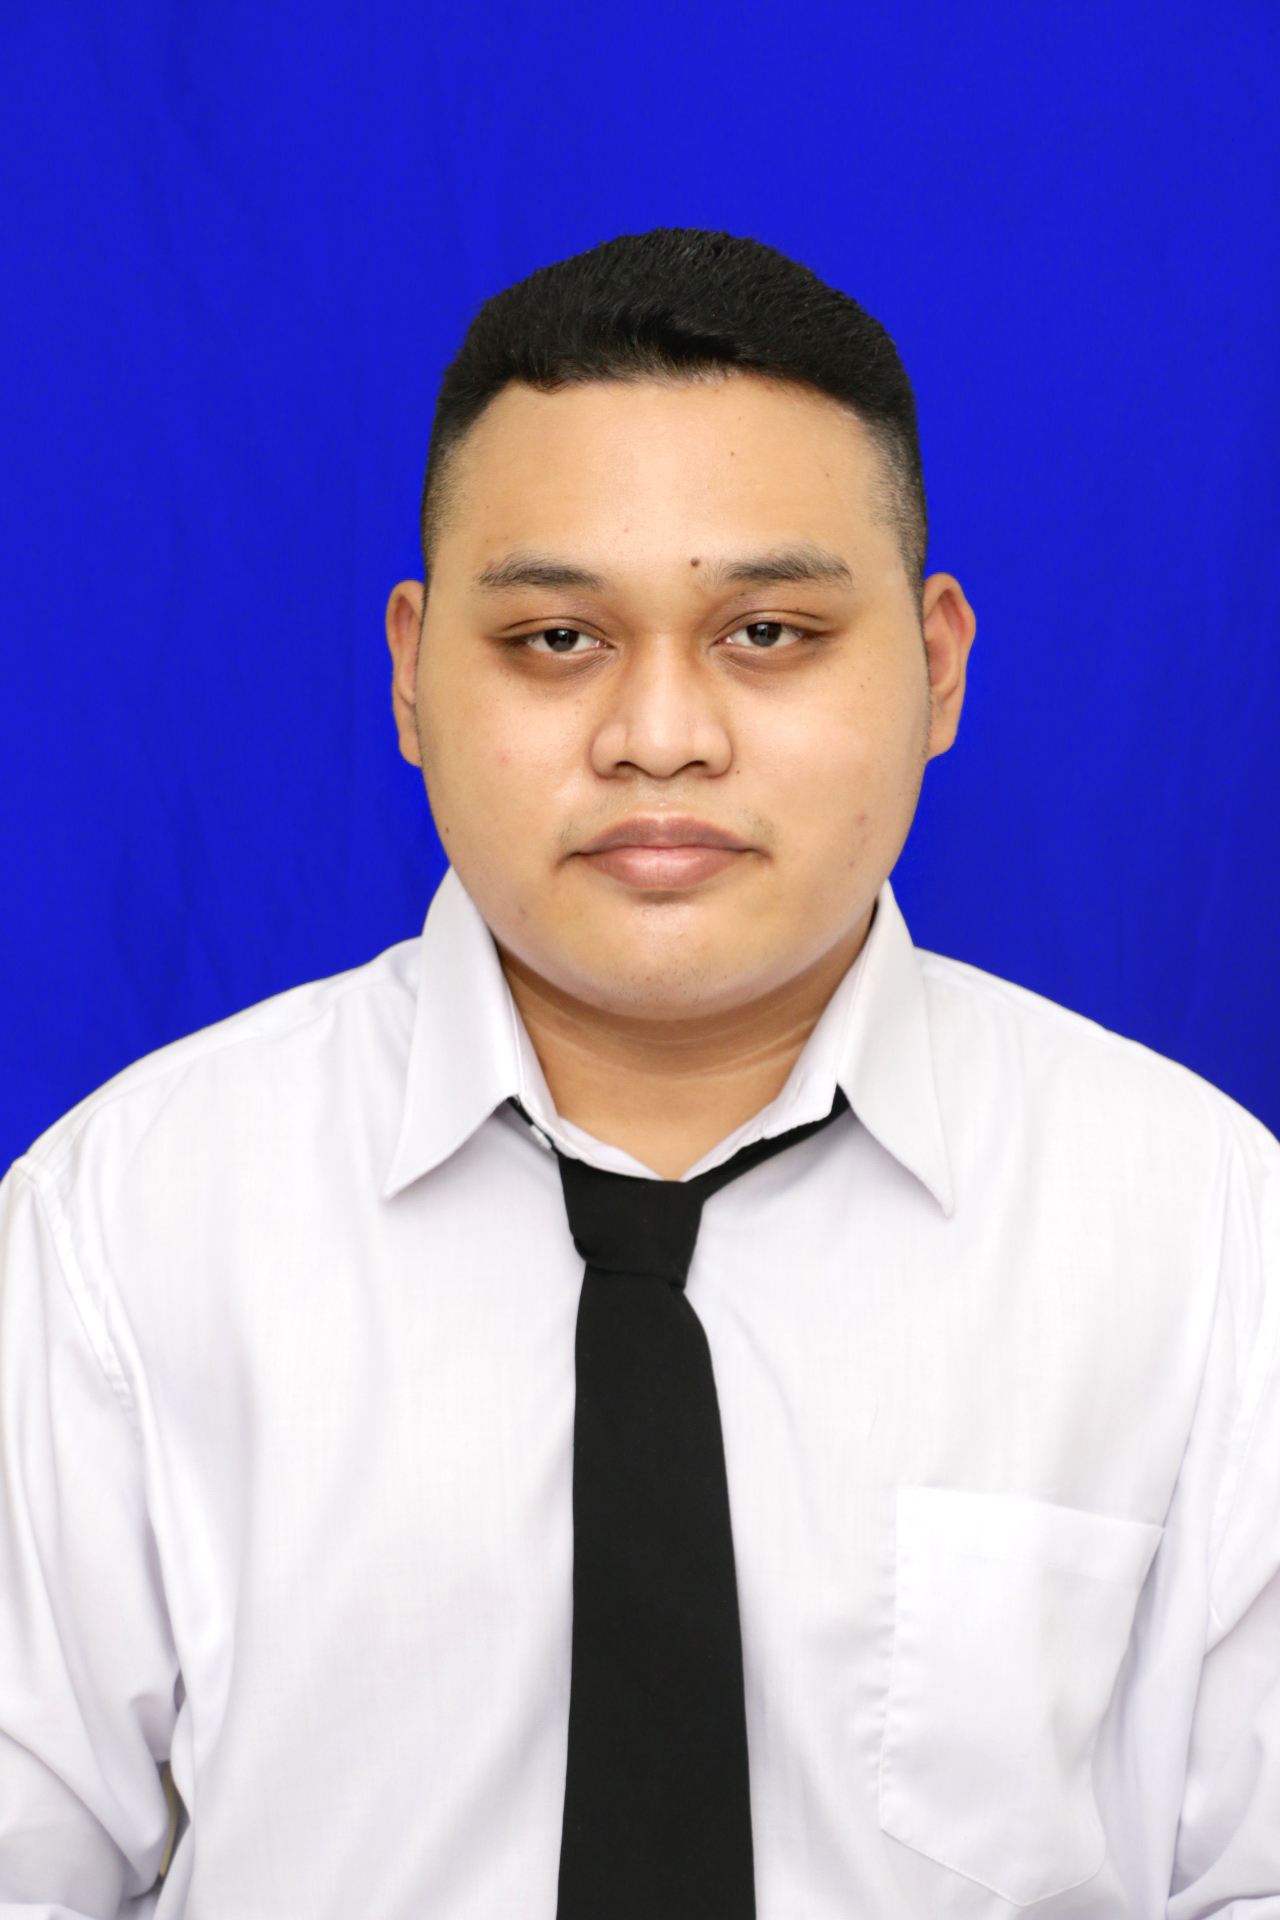
\includegraphics[width=.30\textwidth]{./gambar/Pas Foto Handar Ori.JPG}
    \vspace{-20pt} % Silahkan disesuaikan apabila space di bawah gambar terlalu kecil/besar
  \end{center}
\end{wrapfigure}

\noindent Nama lengkap penulis Hanandaru Mahaputra Purwanto, dengan nama panggilan Handar. Penulis dilahirkan di Surabaya, 23 September 2002, merupakan anak pertama dari dua bersaudara. Penulis telah menempuh pendidikan formal di SMPK Tegaljaya Badung dan SMAK Kolese Santo Yusup Malang. Setelah lulus dari SMA pada tahun 2021 penulis diterima di Departemen Fisika FSAD-ITS dan terdaftar sebagai mahasiswa dengan NRP 5001211007. Selama duduk di bangku kuliah penulis aktif mengikuti kegiatan perkuliahan. Di Departemen Fisika ITS, penulis mengambil bidang studi fisika material. Penulis pernah menjadi asisten laboratorium mata kuliah Fisika Mekanika dan Fisika Listrik dan Magnet. Penulis memiliki ketertarikan pada bidang simulasi sistem kuantum, fisika zat mampat, dan DFT.
 
\vspace{7pt}
\noindent Email: \emailMahasiswa

%======================================================================
    
%=====================================================================
\end{document}
%=====================================================================

%%%%%%%%%%%%%%%%%%%%%%%%%%%%%%%%%%%%%%%%%%%%%%%%%%%%%%%%%%%%%%%%%%%%%%